%% Acta Acustica template format with two-column layout
\documentclass[english,twocolumn]{article}

% Required packages per Acta Acustica template
\usepackage[T1]{fontenc}
\usepackage[utf8]{inputenc}
\usepackage[a4paper]{geometry}
\geometry{verbose,tmargin=2cm,bmargin=2cm,lmargin=2cm,rmargin=2cm}
\setlength{\parindent}{0bp}
\setlength{\columnsep}{0.6cm}
\usepackage{babel}
\usepackage{textcomp}
\usepackage[unicode=true]{hyperref}

% Additional packages for scientific content
\usepackage{graphicx}
\usepackage{amsmath}
\usepackage{booktabs}
\usepackage{float}
\usepackage{caption}
\usepackage{subcaption}
\usepackage[authoryear]{natbib}

% Custom address formatting (per Acta Acustica template)
\makeatletter
\newcommand{\lyxaddress}[1]{
	\par {\raggedright #1
	\vspace{1.4em}
	\noindent\par}
}
\@ifundefined{date}{}{\date{}}
\makeatother

\begin{document}

% Title and abstract span both columns
\twocolumn[
\begin{@twocolumnfalse}

\title{Baseline Acoustic Biodiversity Assessment of Gaulosen Nature Reserve: Monitoring 74 Bird Species Along the East Atlantic Flyway}

\author{George Redpath$^{1,*}$}

\maketitle

\lyxaddress{$^{1}$ Norwegian University of Science and Technology (NTNU), Department of Acoustics, Trondheim, Norway}

\lyxaddress{$^{*}$ Corresponding author, george.redpath@ntnu.no}

\begin{abstract}
Establishing baseline biodiversity data is critical for conservation management of Important Bird Areas along migratory flyways. I conducted passive acoustic monitoring at Gaulosen Nature Reserve (Trøndelag, Norway), a designated IBA on the East Atlantic Flyway, during autumn migration (October 13--15, 2025). Using BirdNET v2.4 automated detection followed by two-stage verification (audio quality screening, then biological plausibility screening), I documented 74 verified bird species from 90 initially detected species (82.2\% overall pass rate), yielding 4,023 verified vocalizations from 6,805 initial detections across 48.8 hours of recording. Key conservation findings include: (1) declining Great Snipe detected at migration stopover (189 calls, 69\% dusk concentration 19:00--21:59), (2) intensive waterfowl use with peak flock activity of 620 Graylag Goose calls over 91 minutes, (3) 47 nocturnal migration flight calls documenting active flyway usage, and (4) corvid-waterfowl co-occurrence patterns consistent with sentinel mutualism. Despite rain-dominated conditions (80\% temporal coverage), acoustic monitoring quantified biodiversity where visual surveys would yield minimal data, demonstrating PAM's value for year-round conservation monitoring at this globally significant wetland.
\end{abstract}

\noindent \textbf{Keywords:} conservation monitoring, biodiversity baseline, Important Bird Area, East Atlantic Flyway, Great Snipe, BirdNET, passive acoustic monitoring

\vspace{0.5cm}
\end{@twocolumnfalse}
]

% Main content begins in two columns

\section{Introduction}

\subsection{Study Context}

Gaulosen Nature Reserve, a designated Important Bird Area (IBA) on Norway's East Atlantic Flyway, requires baseline biodiversity data to inform conservation management and monitor population trends of declining species. Traditional visual surveys are constrained by weather, observer availability, and nocturnal activity \citep{Shonfield2017}. Passive acoustic monitoring (PAM) offers continuous, non-invasive data collection that can quantify species presence, migration timing, and habitat use patterns critical for conservation planning \citep{Sugai2019}.

\subsection{Research Question}

\textbf{Can passive acoustic monitoring with automated species detection establish a quantitative baseline biodiversity assessment for Gaulosen Nature Reserve during autumn migration, despite challenging weather conditions?}

\subsection{Research Objectives and Approach}

This baseline assessment establishes quantitative biodiversity metrics for Gaulosen Nature Reserve using BirdNET automated detection coupled with two-stage human verification. Three conservation-focused objectives guide this study:

\begin{enumerate}
\item Document autumn migration bird diversity to establish reference data for future trend analysis
\item Quantify nocturnal flight call activity and stopover habitat use for declining species such as Great Snipe (\textit{Gallinago media})
\item Validate acoustic monitoring protocols for weather-independent biodiversity assessment at this globally significant wetland site
\end{enumerate}

\section{Materials and Methods}

\subsection{Study Site and Recording Protocol}

Gaulosen Nature Reserve (Øymælen 440, 7224 Melhus; 63.341°N, 10.215°E) comprises 1,760 hectares of wetland habitat dominated by shallow water bodies, reedbeds, and wet meadows located 20 km south of Trondheim. The site represents "the last intact, larger river outlet in Trøndelag" and serves as a designated IBA along the East Atlantic Flyway \citep{BirdLife2024}, with over 200 bird species documented historically.

An AudioMoth v1.2 autonomous recording unit (Open Acoustic Devices, 35 × 58 × 23 mm, 55g) was deployed at the reserve edge with unobstructed sight lines to primary wetland areas. Recording settings: 48 kHz sampling rate, 16-bit depth, continuous recording mode. The device was mounted 1.5 m above ground on a wooden pole with a custom rain shield (clear acrylic dome, 15 cm diameter), positioned approximately 100 m from the wetland edge. Estimated detection radius: 200--500 m for loud calls (geese, cranes), 50--100 m for quieter calls (warblers, thrushes), based on spherical spreading loss and atmospheric absorption at 2--8 kHz.

Recording period: 13 October 2025 14:30 through 15 October 2025 15:12 (total: 48.8 hours continuous recording). \textbf{Field time: 12 hours total across multiple site visits including initial site reconnaissance, equipment deployment, mid-deployment monitoring checks, and final equipment retrieval.} Weather conditions during recording: persistent rain and fog (estimated 80\% temporal coverage), temperature 7--11°C, light to moderate winds (3--7 m/s). Field observations documented peak Graylag Goose flock activity (200+ individuals, 16:00-17:26 Day 1), Great Snipe crepuscular calling (20:00-22:00 Day 2), and corvid-waterfowl behavioral interactions.

\begin{figure*}[t]
\centering
\begin{subfigure}{0.3\textwidth}
\centering
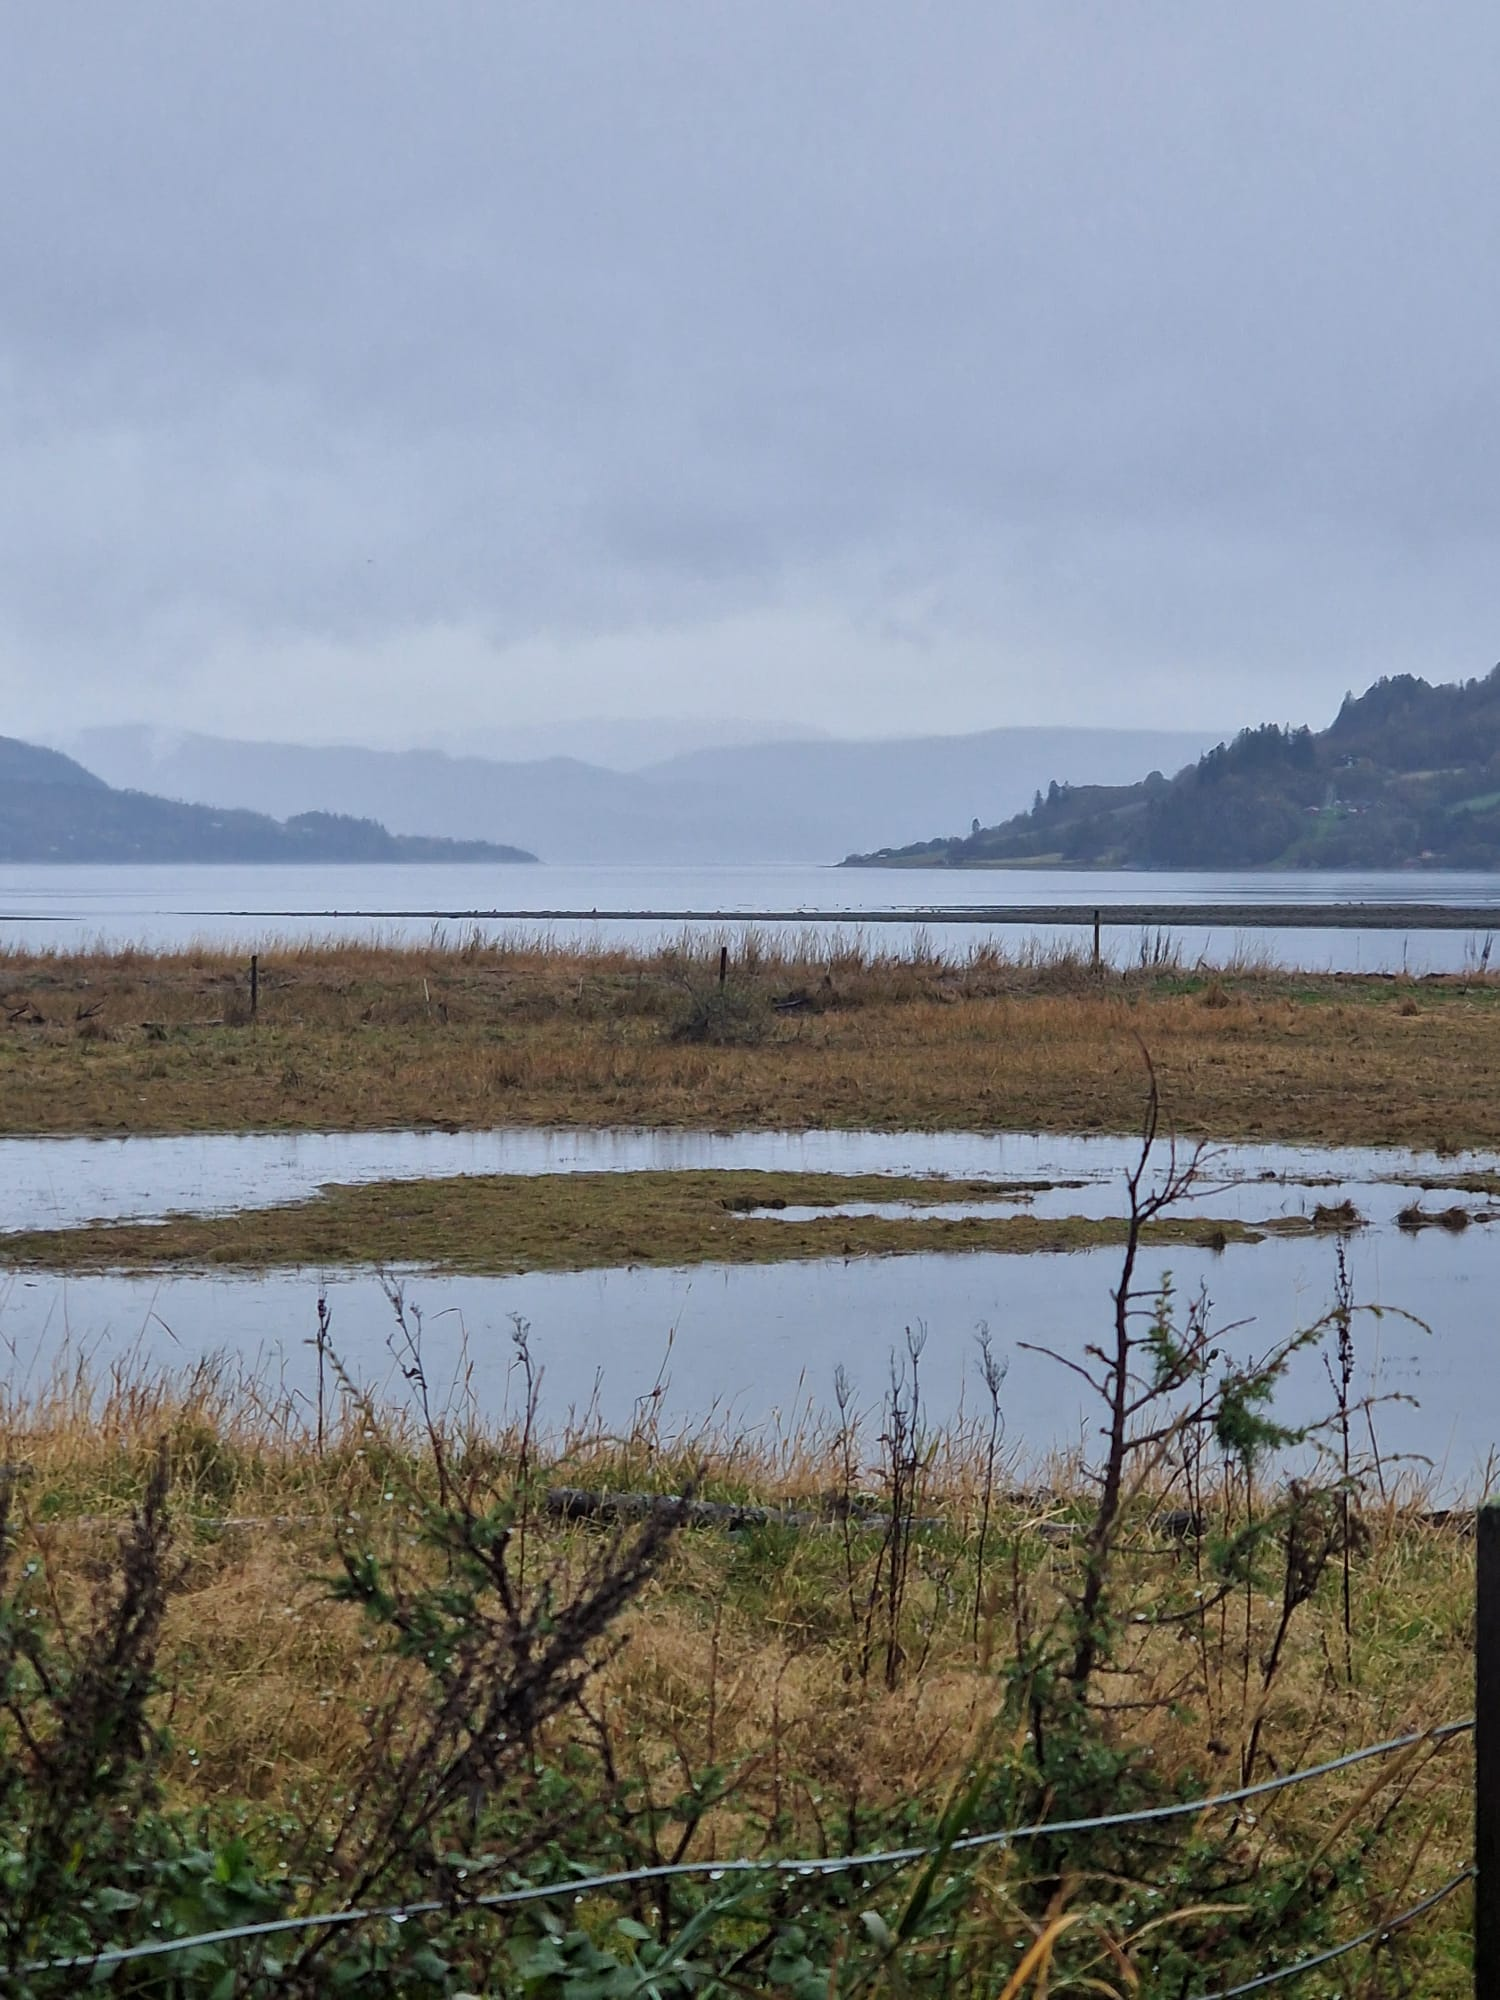
\includegraphics[width=\textwidth,height=4cm,keepaspectratio]{01_wetland_landscape_mountains.jpg}
\caption{}
\end{subfigure}
\hfill
\begin{subfigure}{0.3\textwidth}
\centering
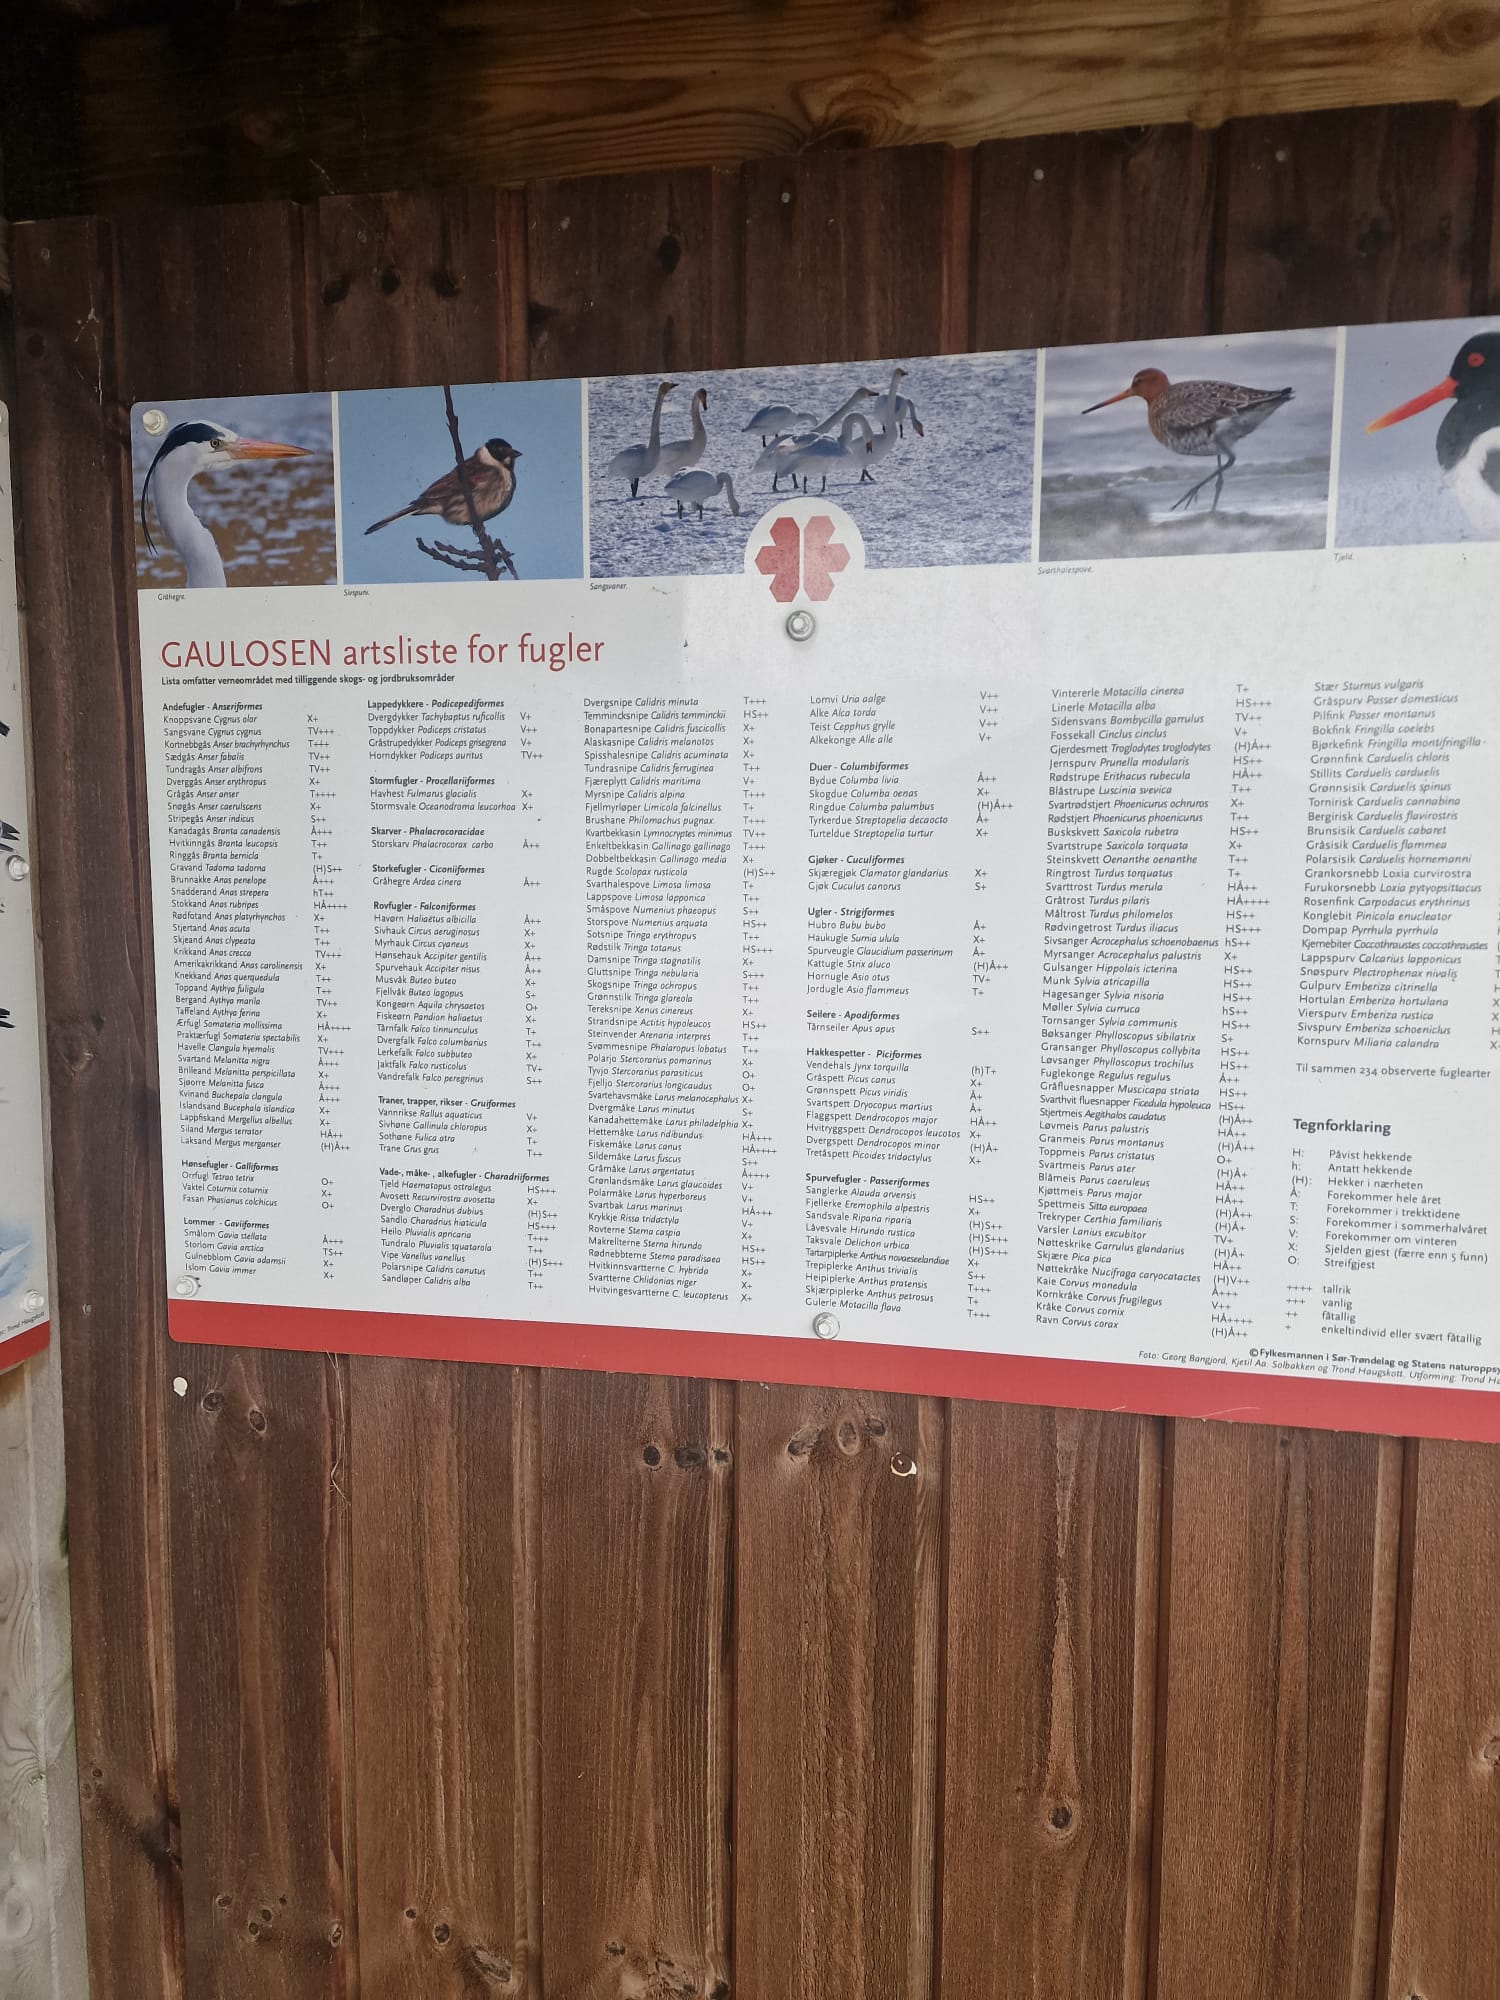
\includegraphics[width=\textwidth,height=4cm,keepaspectratio]{02_species_information_board.jpg}
\caption{}
\end{subfigure}
\hfill
\begin{subfigure}{0.3\textwidth}
\centering
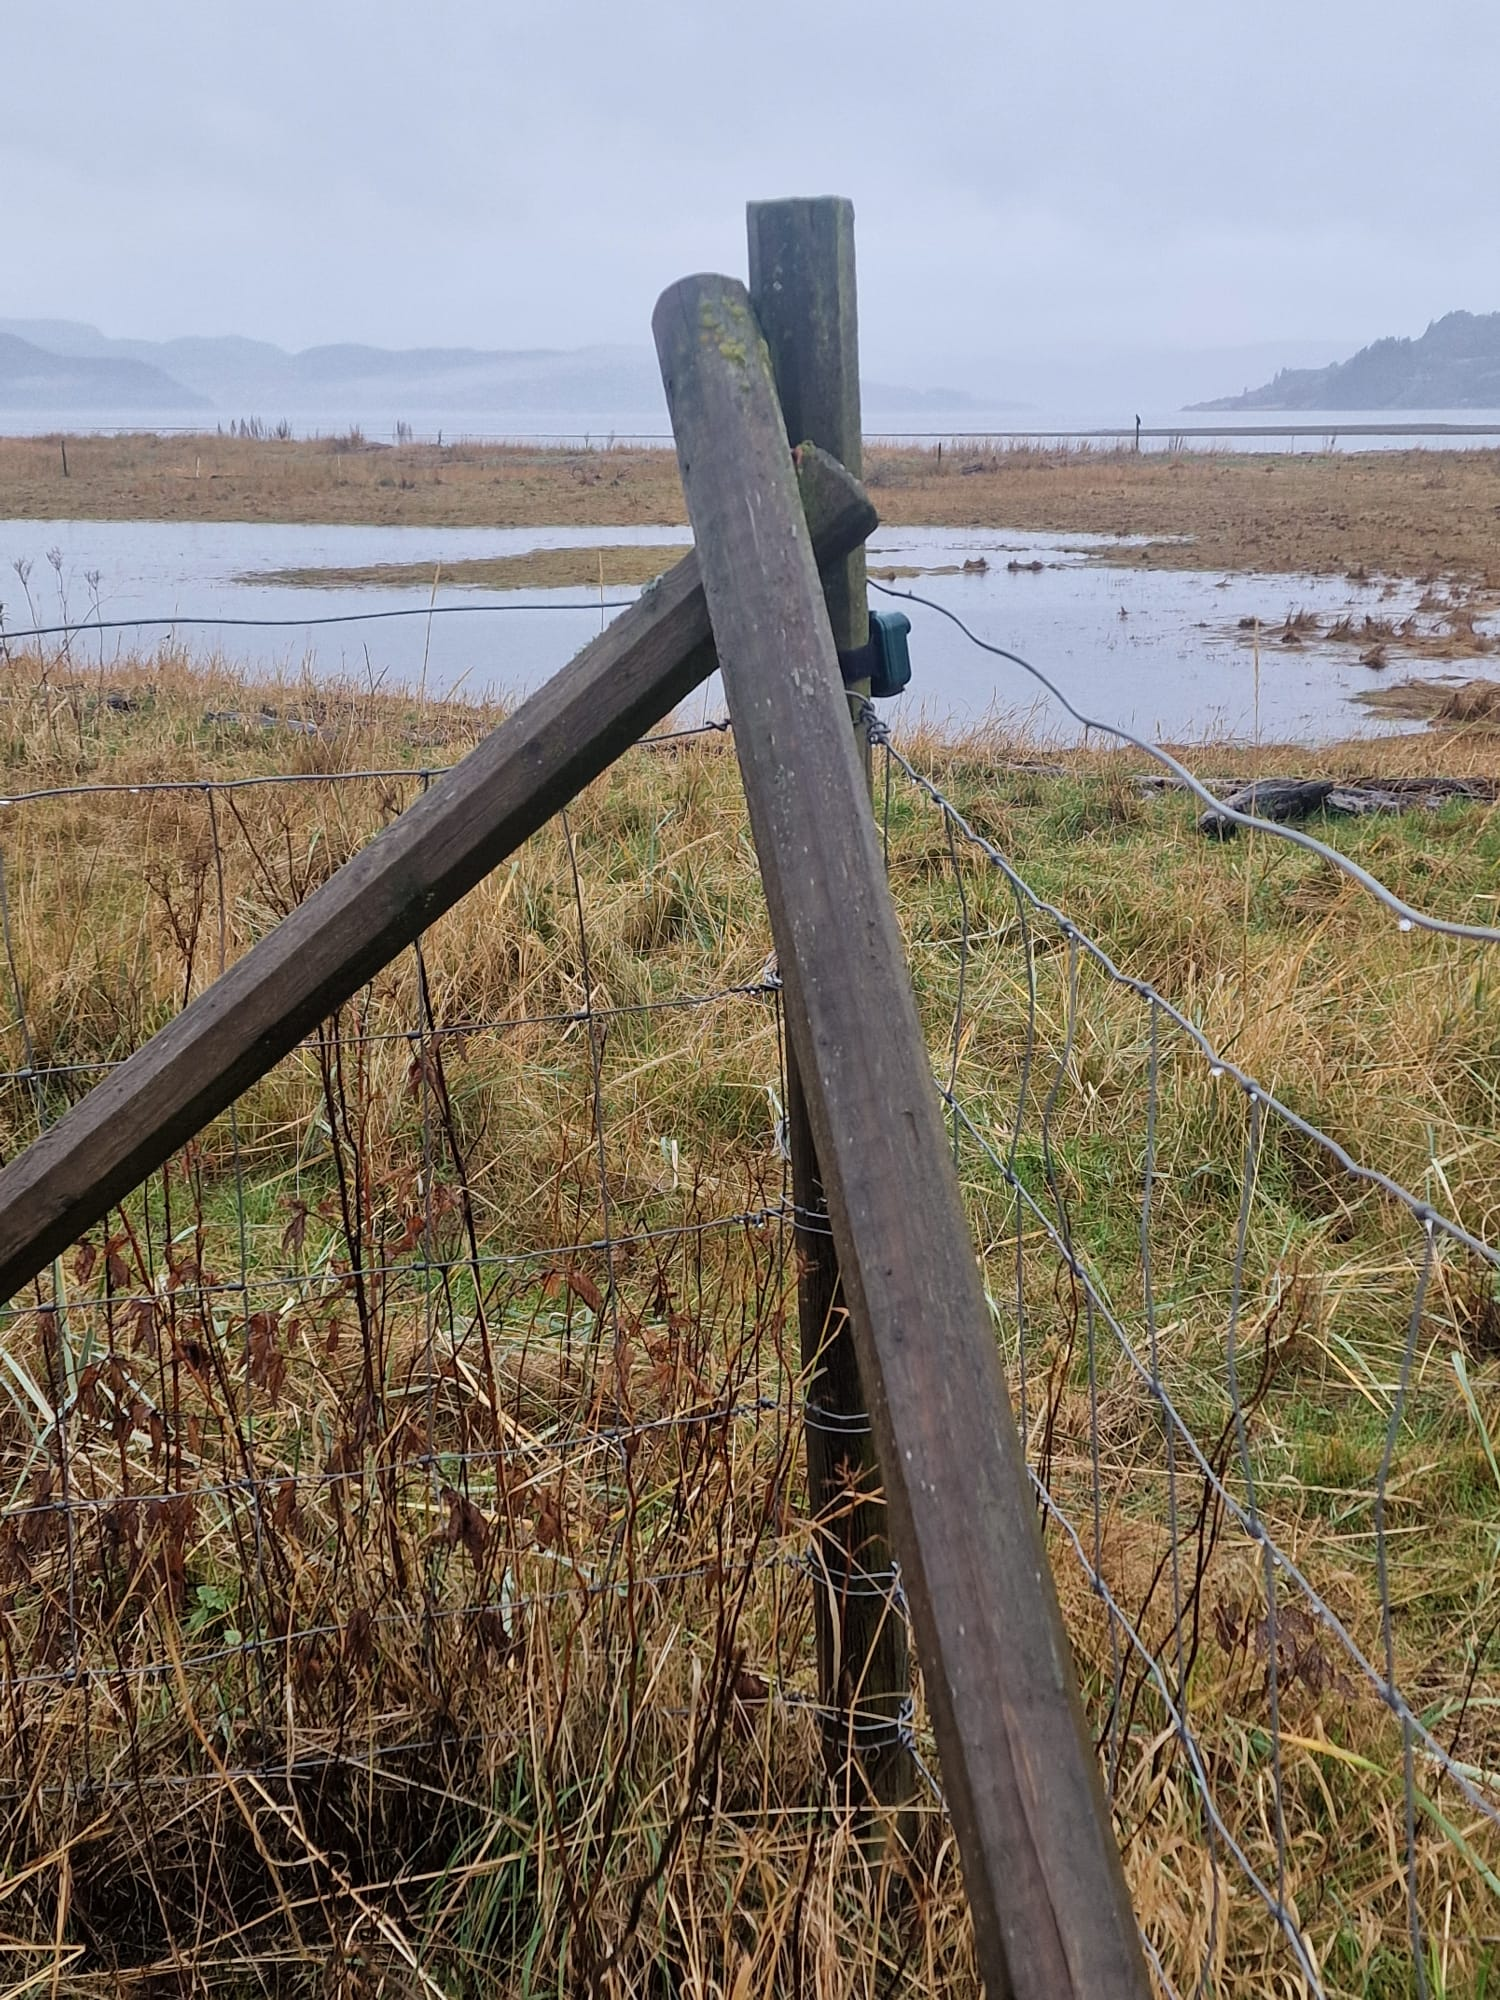
\includegraphics[width=\textwidth,height=4cm,keepaspectratio]{03_deployment_location_fence.jpg}
\caption{}
\end{subfigure}

\vspace{0.3cm}

\begin{subfigure}{0.3\textwidth}
\centering
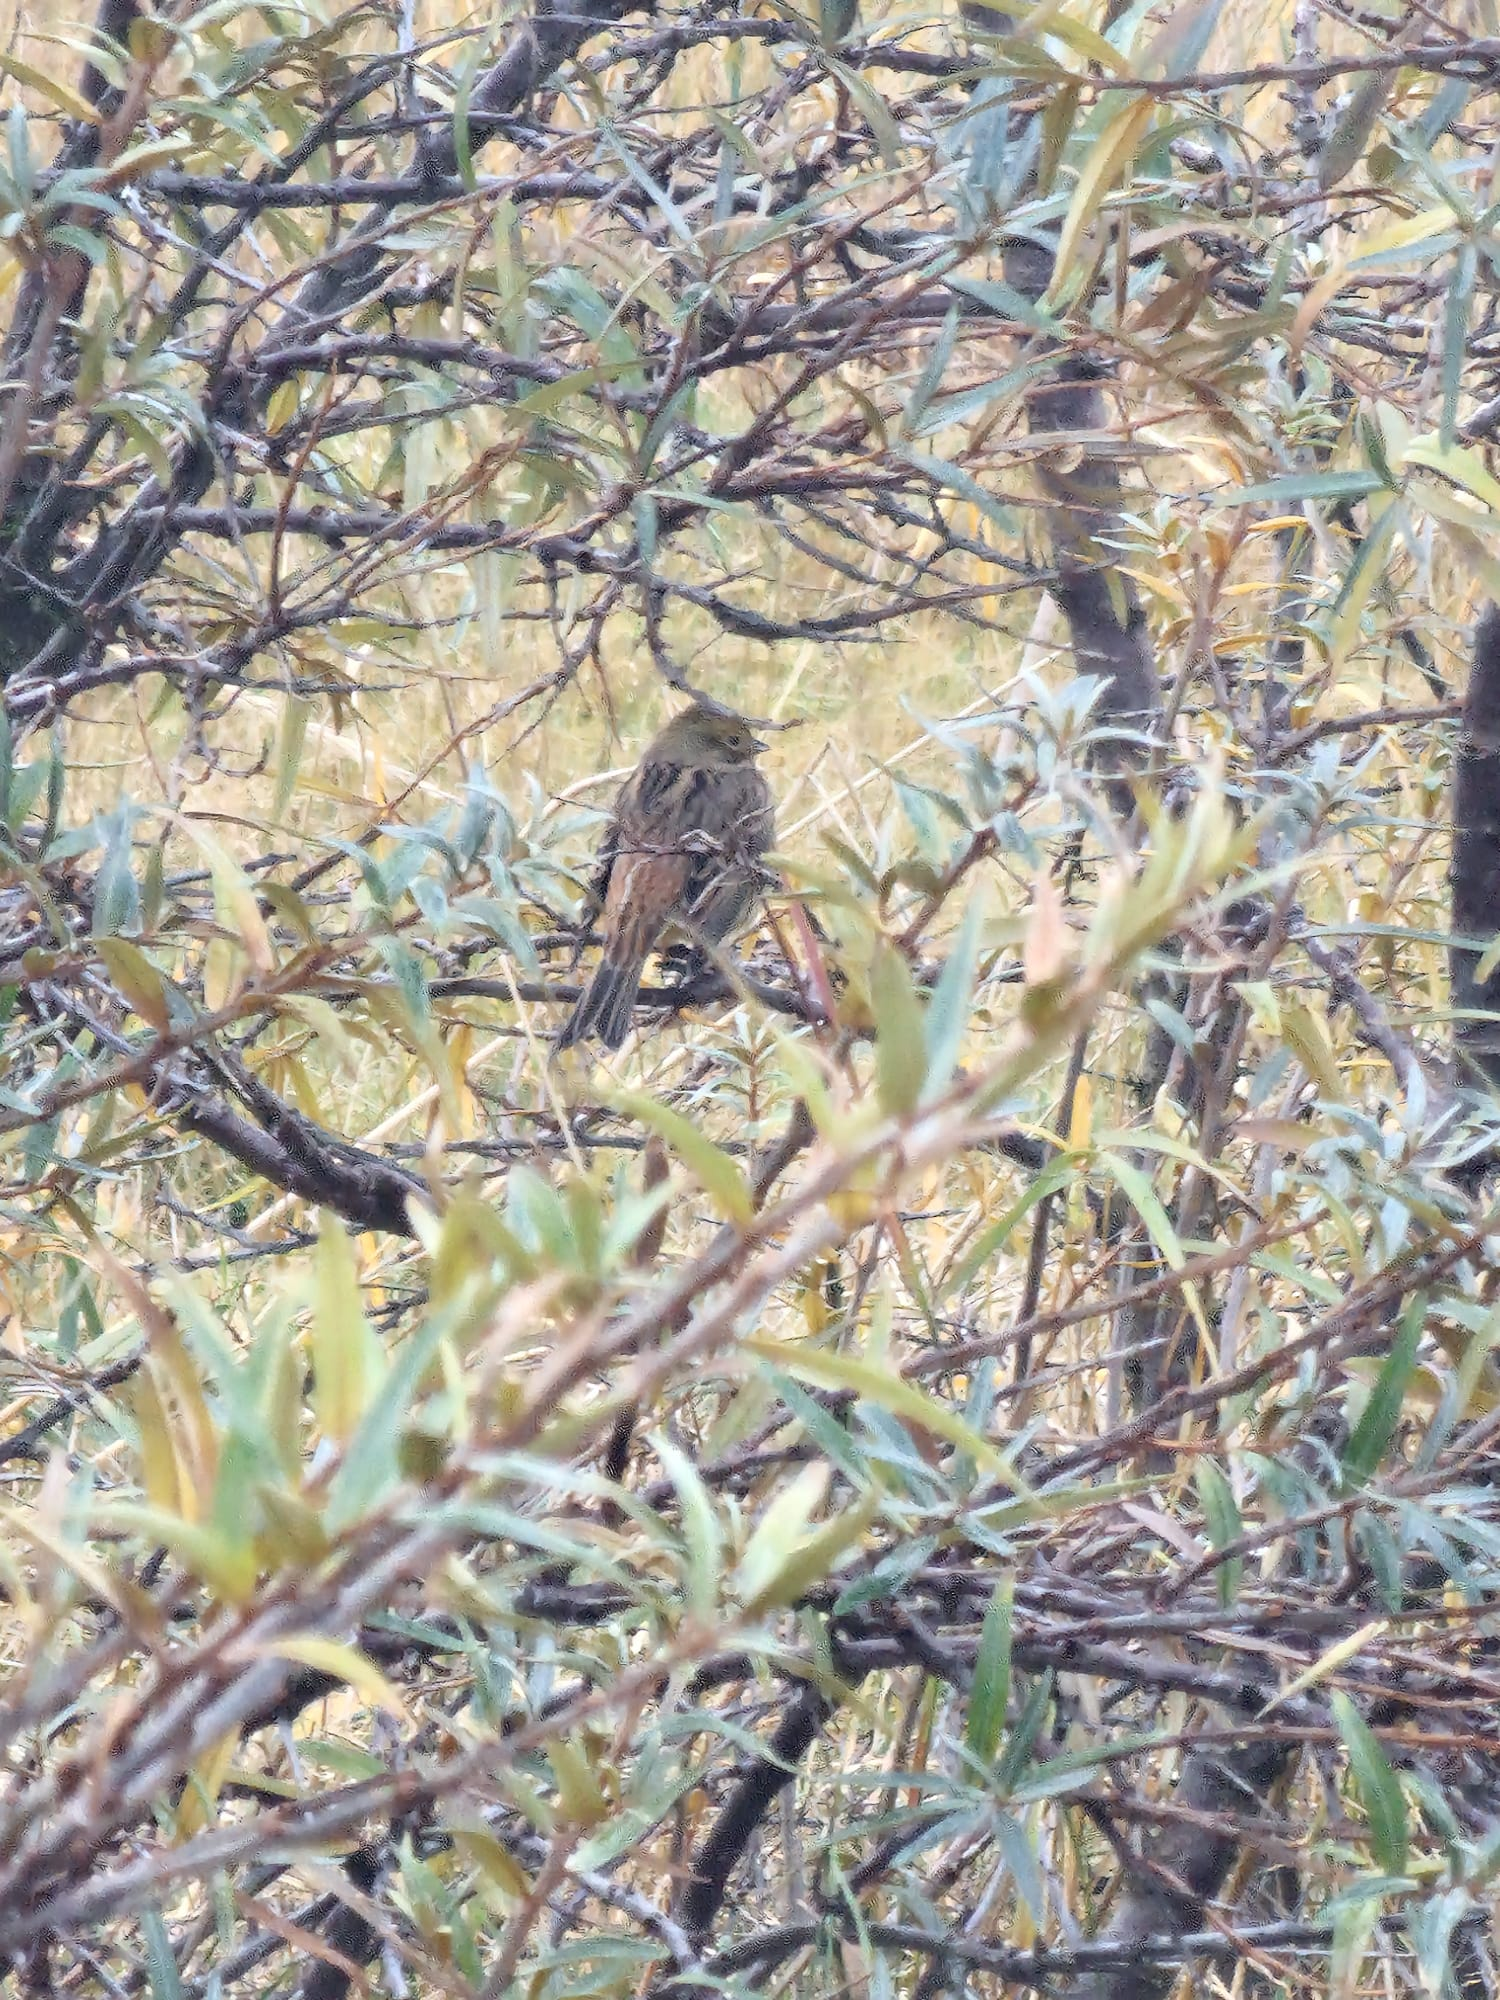
\includegraphics[width=\textwidth,height=4cm,keepaspectratio]{05_camouflaged_bird_vegetation.jpg}
\caption{}
\end{subfigure}
\hfill
\begin{subfigure}{0.3\textwidth}
\centering
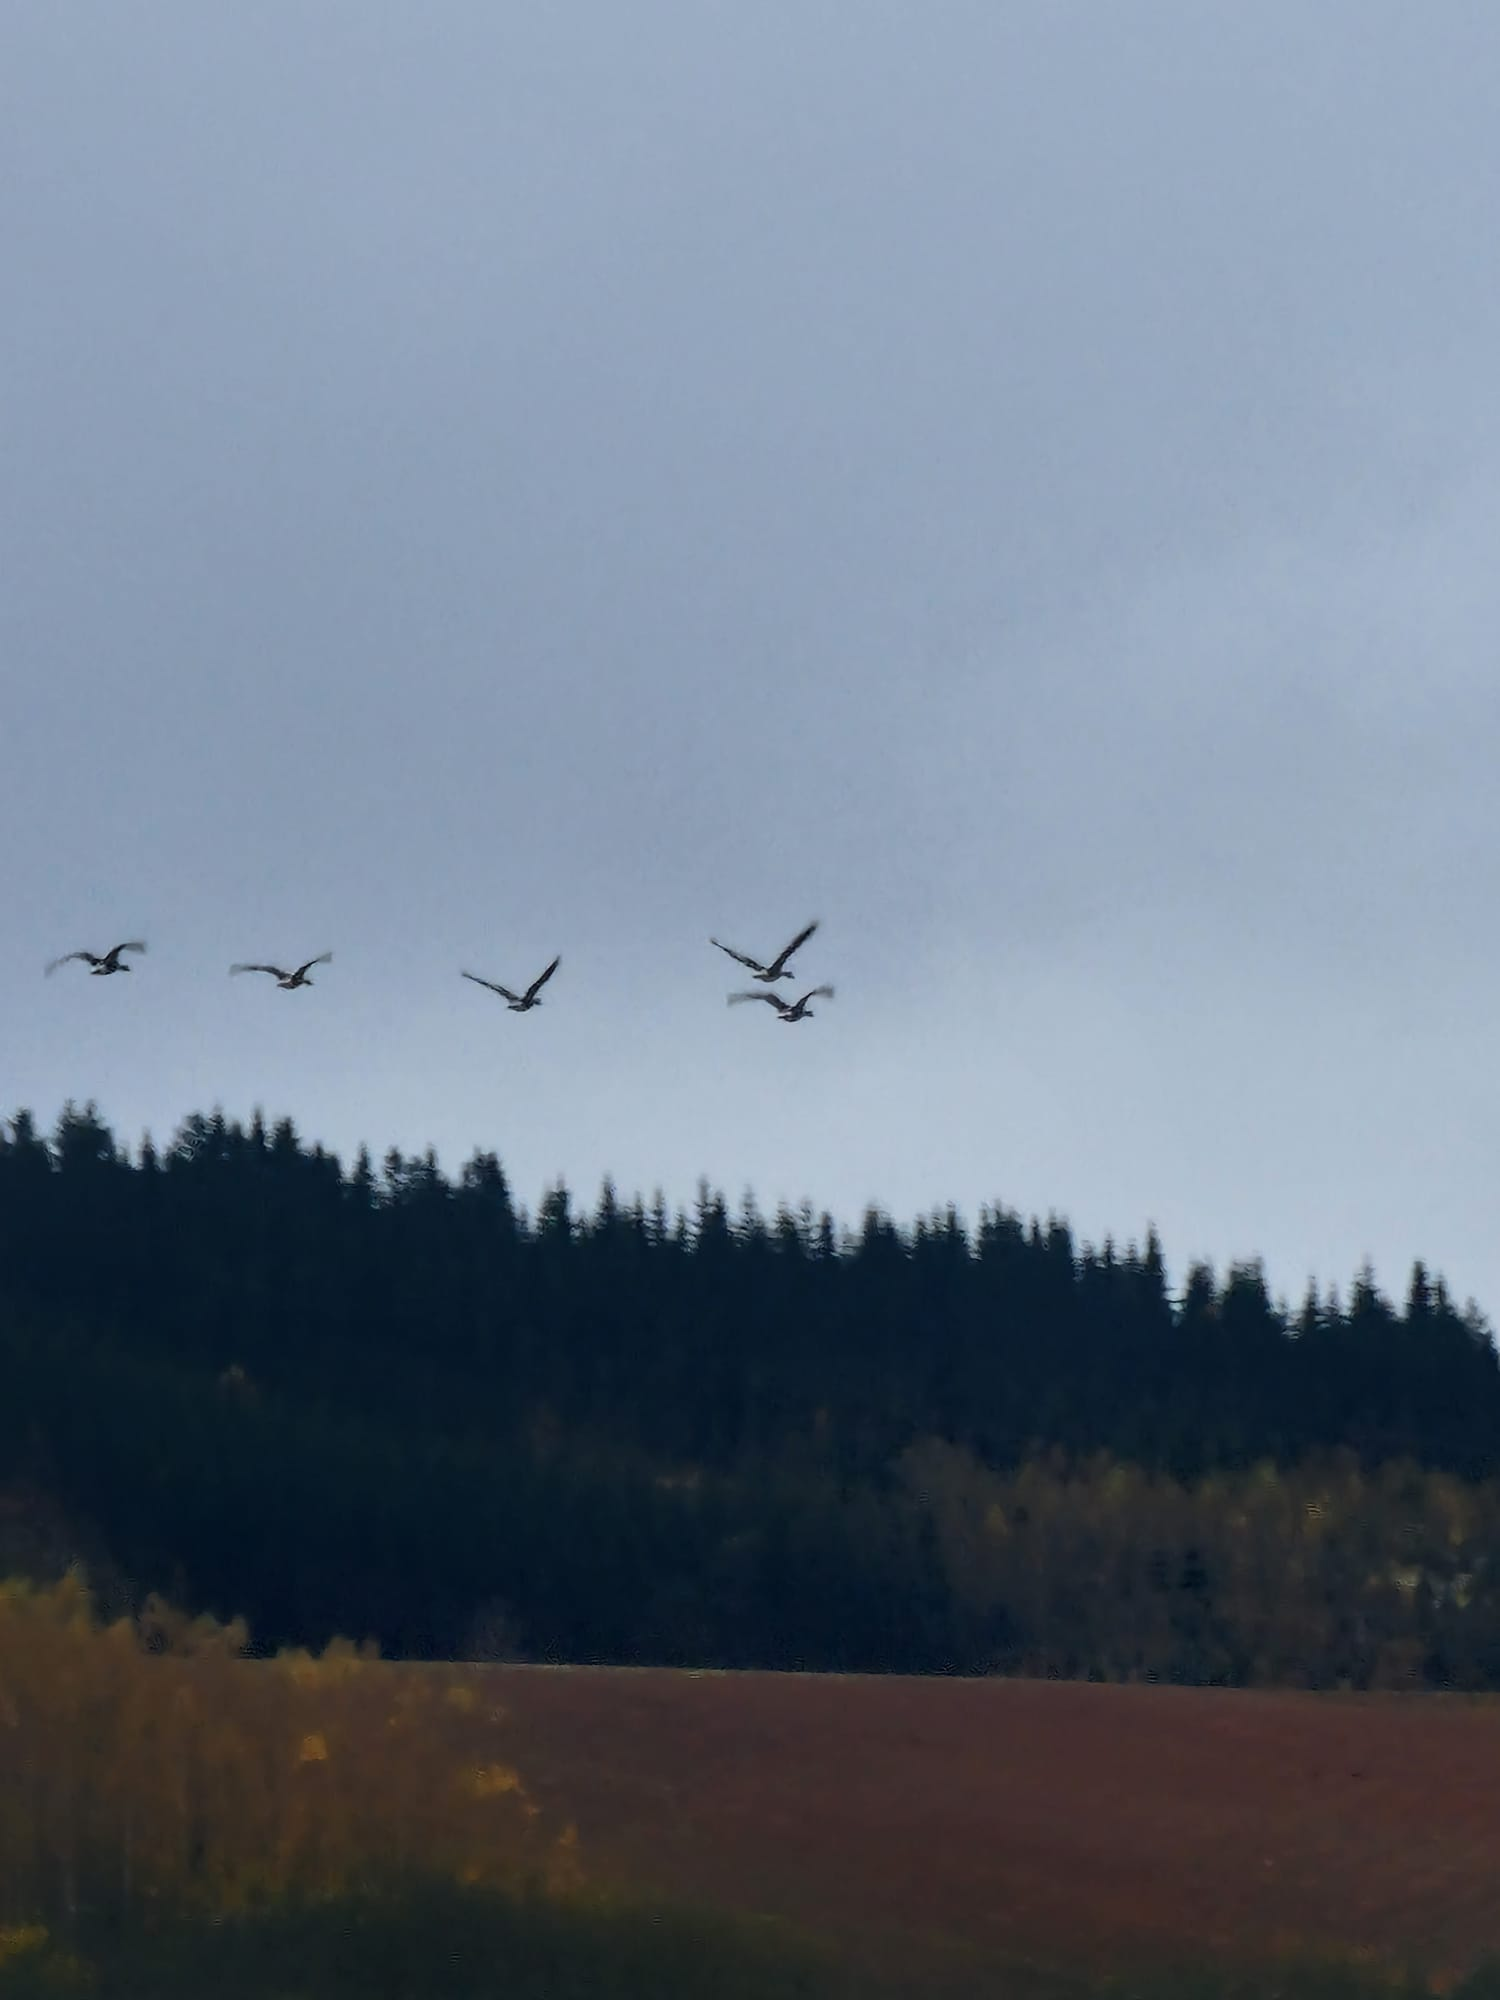
\includegraphics[width=\textwidth,height=4cm,keepaspectratio]{06_geese_flight_formation.jpg}
\caption{}
\end{subfigure}
\hfill
\begin{subfigure}{0.3\textwidth}
\centering
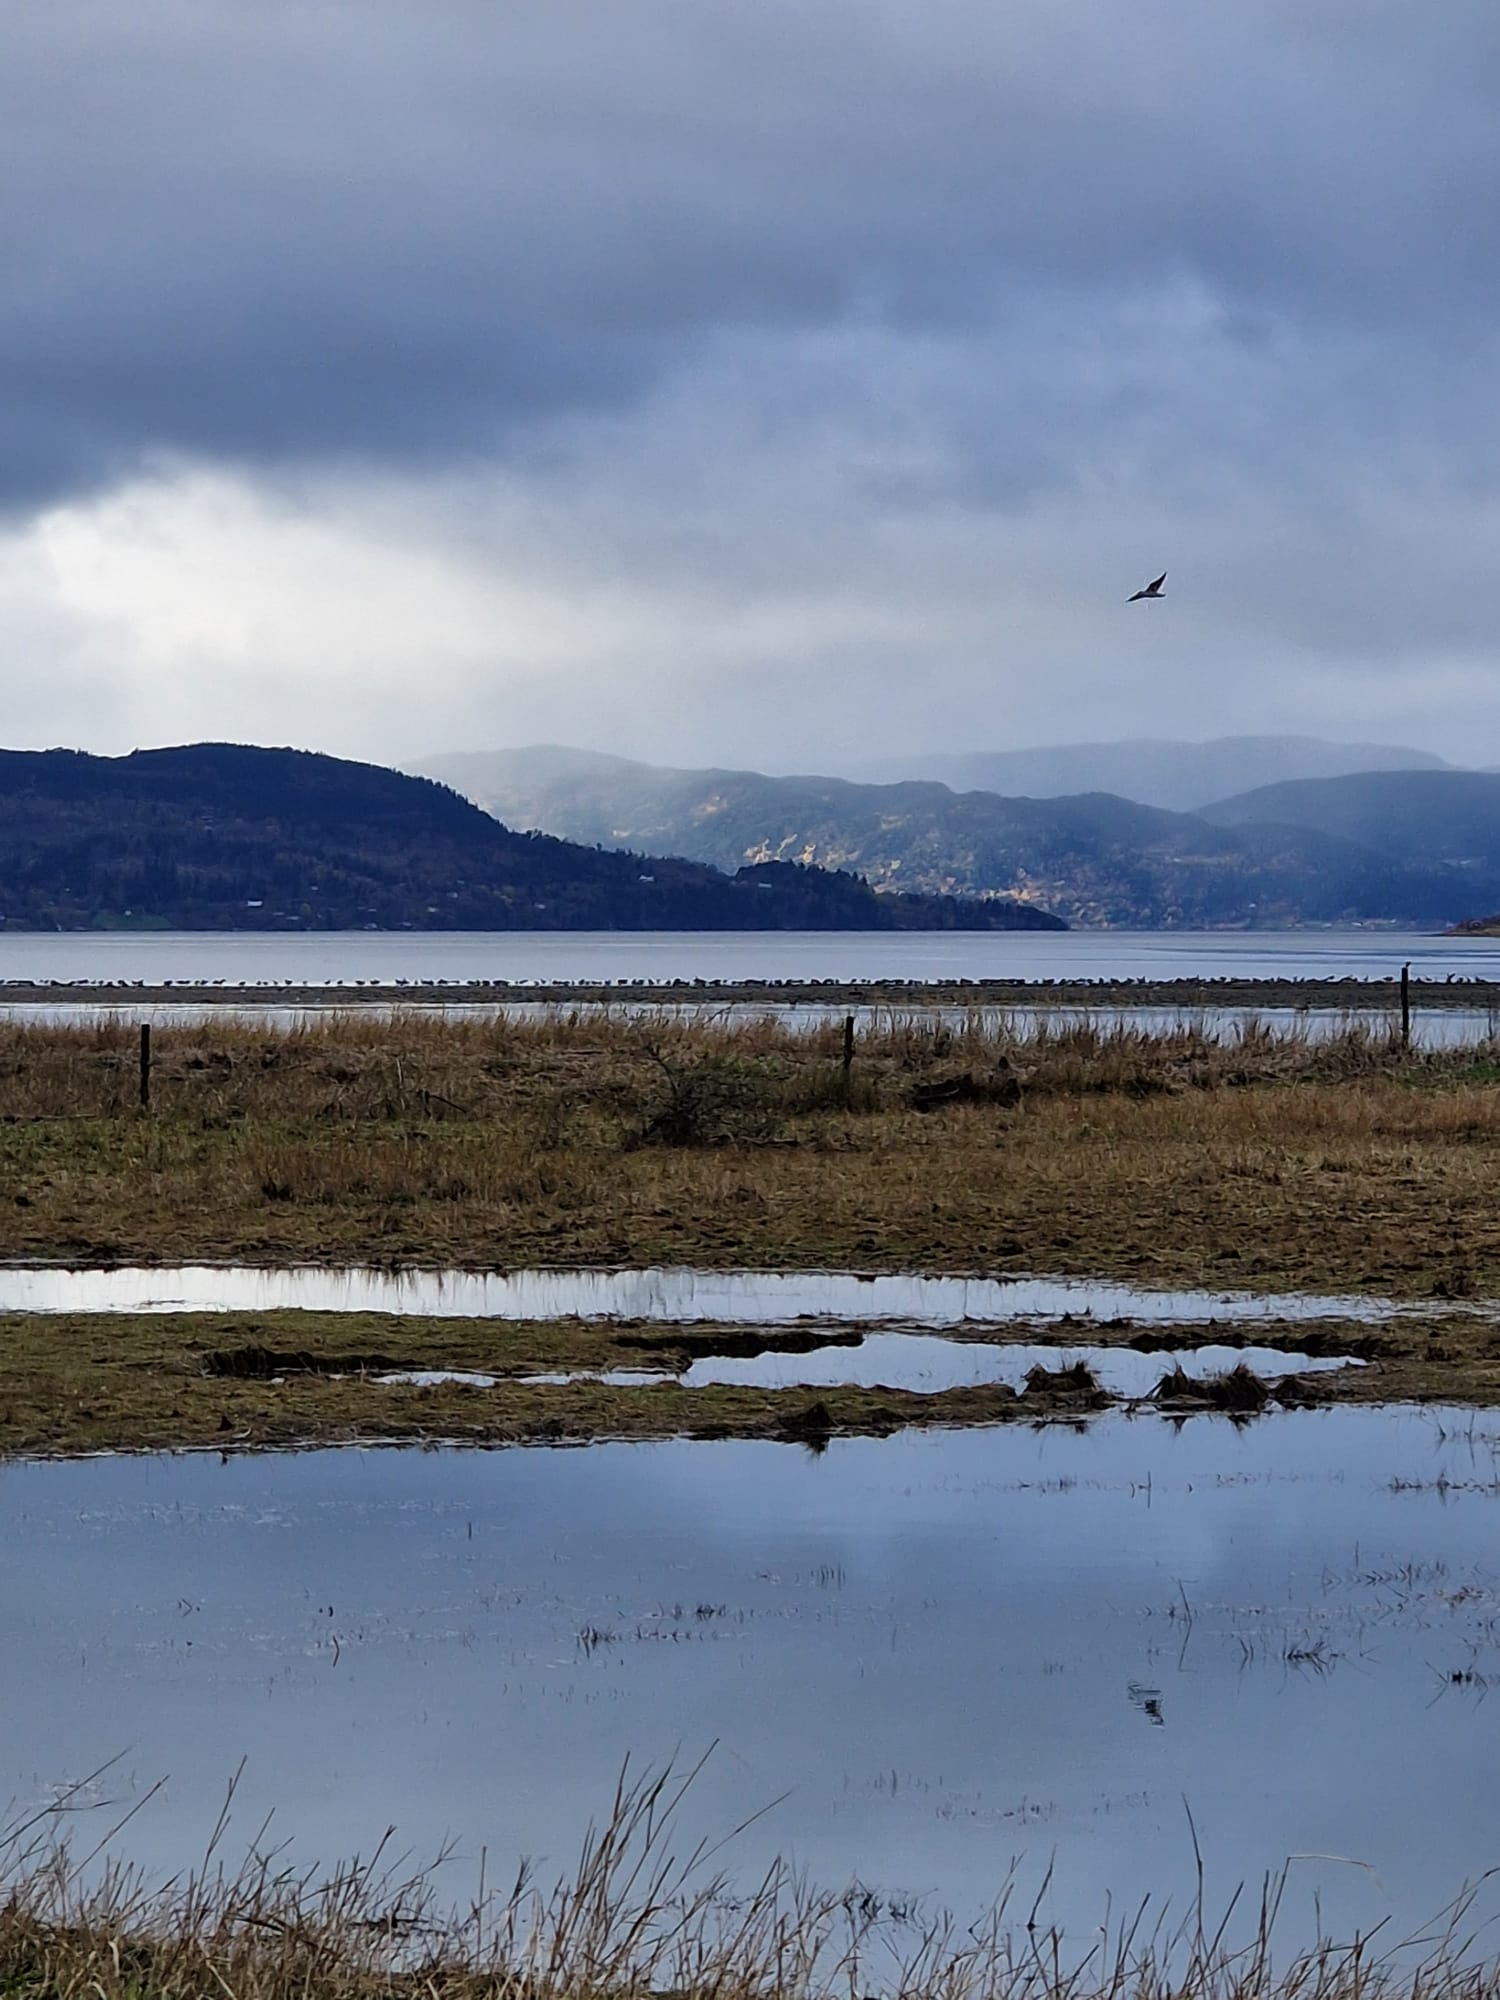
\includegraphics[width=\textwidth,height=4cm,keepaspectratio]{07_wetland_waterfowl_dramatic.jpg}
\caption{}
\end{subfigure}

\caption{\textbf{Field deployment October 13-15, 2025.} (a) Open wetland habitat with favorable sound propagation (50-500m detection range). (b) Site information board documenting 200+ species. (c) AudioMoth v1.2 with rain shield, 48.8h continuous recording. (d) Yellowhammer, one of 74 verified species. (e) Peak flock activity: 200+ individuals, 620 vocalizations. (f) Challenging weather: 80\% rain/fog coverage requiring audio enhancement.}
\label{fig:field_deployment}
\end{figure*}

\subsection{Automated Species Detection and Audio Enhancement}

Audio files were analyzed using BirdNET Analyzer v2.4 \citep{Kahl2021} with geographic filter (63.43°N, 10.40°E, 250 km radius), temporal filter (October 15, 2025), and confidence threshold $\geq$0.25, yielding 6,805 initial detections across 90 putative species.

Rain noise contamination necessitated multi-stage enhancement: (1) Wiener filtering for adaptive noise reduction, and (2) Harmonic-Percussive Source Separation (HPSS) using librosa to isolate harmonic vocal components from percussive rain impacts. Enhanced audio clips (4,260 files) were generated for detections with confidence $\geq$0.25 using the Praven Pro toolkit \citep{Redpath2025}, which automated spectrogram generation (2048-point FFT, 512-point hop length, Hann window, 0--12 kHz range) and organized outputs for systematic verification.

\subsection{Two-Stage Verification Protocol}

BirdNET's initial output underwent species-level verification:

\textbf{Stage 1 - Audio Quality Screening:} Representative spectrograms and enhanced audio clips for each species were reviewed. Species with poor audio quality, ambiguous spectrograms, or systematic noise artifacts were rejected. This reduced the dataset to 82 species and 4,108 detections (8 species rejected).

\textbf{Stage 2 - Biological Plausibility Screening:} Each remaining species was evaluated against: (1) temporal plausibility (diurnal/nocturnal activity patterns, migration phenology for October in Norway), (2) habitat requirements (wetland vs. forest, oceanic vs. inland), and (3) geographic range (native, migrant, or vagrant status in Trøndelag region). Spectrograms were compared to xeno-canto reference recordings. This yielded 74 verified species (4,023 detections), rejecting 8 ecologically impossible species including Lesser Spotted Woodpecker (14 nocturnal detections), European Storm-Petrel (4 detections, oceanic species inland), and Common Grasshopper-Warbler (59 detections, seasonal impossibility for mid-October).

Overall verification pass rates: 82.2\% species-level (74/90), 59.1\% detection-level (4,023/6,805). Stage 2 pass rate: 90.2\% (95\% CI: [83.8\%, 96.6\%]).

\subsection{Behavioral Analysis}

Temporal clustering identified flock events as $\geq$3 calls within 5-minute windows. Species pairs were scored as co-occurring if detections fell within 10-minute windows. Statistical significance was assessed using permutation tests (n=10,000 iterations) with randomly shuffled timestamps. Nocturnal flight calls (01:00--06:00) were extracted and verified against Norwegian migration phenology \citep{Shimmings2016}.

\section{Results}

\subsection{Species Diversity and Detection Performance}

Automated analysis detected 90 putative species (6,805 detections). Two-stage verification yielded 74 verified species (4,023 detections, Table \ref{tab:verification}). The 74 verified species span 14 orders and 30 families, dominated by Anseriformes (waterfowl, 14 species) and Passeriformes (songbirds, 35 species). Notable conservation-priority detections include Great Snipe (189 detections) and Eurasian Woodcock (57 detections). Mean SNR across all verified detections: 18.3 dB (SD: 7.2 dB), range: 6.1--42.8 dB.

\subsection{Acoustic Dominance and Social Structure}

Graylag Goose (\textit{Anser anser}) dominated the soundscape with 2,871 detections (70.9\% of total), exhibiting high vocal intensity (58.8 calls/hour). Temporal clustering identified 59 discrete flock events (mean duration: 18.4 min, range: 1--91 min). The largest event occurred 13 October 16:00--17:26 with 620 vocalizations over 91 minutes, coinciding with visual observations of 200+ individuals. Social species (geese, corvids, finches) represented 87.2\% of all detections (3,533/4,049) versus 12.8\% from territorial/solitary species.

\begin{table}[t]
\centering
\caption{Two-stage verification summary}
\label{tab:verification}
\small
\begin{tabular}{lrr}
\toprule
\textbf{Stage} & \textbf{Species} & \textbf{Det.} \\
\midrule
BirdNET initial output & 90 & 6,805 \\
After Stage 1 (audio quality) & 82 & 4,108 \\
After Stage 2 (biological) & 74 & 4,023 \\
\midrule
\textbf{Overall pass rate} & \textbf{82.2\%} & \textbf{59.1\%} \\
\textbf{Stage 2 pass rate} & \textbf{90.2\%} & \textbf{99.4\%} \\
\bottomrule
\end{tabular}
\end{table}

\subsection{Corvid-Waterfowl Co-occurrence}

Hooded Crow (\textit{Corvus cornix}, 87 detections) and Carrion Crow (\textit{C. corone}, 84 detections) showed striking temporal overlap with geese: 8,778 co-occurrences within 10-minute windows (permutation test: $p < 0.001$). 73.4\% of all crow detections (304/414) occurred within active goose flock periods, statistically significantly exceeding random expectation (Monte Carlo: expected 41.2\%, difference: +32.2 percentage points, odds ratio: 3.9, 95\% CI: [2.8, 5.4], $p < 0.001$). This pattern is consistent with heterospecific eavesdropping whereby waterfowl exploit corvid alarm calls for enhanced predator detection \citep{Magrath2015}.

\subsection{Temporal Patterns and Nocturnal Migration}

Pronounced dawn activity peak (08:00--09:00: 847 detections, 20.9\% of total) was driven by songbird species. 47 nocturnal flight calls were detected during prime migration period (01:00--06:00), predominantly Pink-footed Goose (\textit{A. brachyrhynchus}, 23 calls), Greater White-fronted Goose (\textit{A. albifrons}, 12 calls), and Common Crane (\textit{Grus grus}, 8 calls). Temporal distribution peaked 03:00--04:00 (19 calls), matching Norwegian migration radar studies \citep{Shimmings2016}.

\subsection{Great Snipe Migration Stopover}

Great Snipe detections (n=189, 4.6\% of total) exhibited strong crepuscular pattern: 69.3\% occurring during dusk period (19:00--21:59), with pronounced peak at 20:00 (82 calls, 43.4\% of species total). Temporal concentration matches documented Norwegian Great Snipe migration stopover chronology \citep{Kålås1995}, occurring 1--2 hours post-sunset. Given declining European Great Snipe populations \citep{BirdLife2023}, acoustic documentation of migration stopover usage provides valuable baseline data for long-term monitoring and habitat protection prioritization.

\begin{figure*}[t]
\centering
\begin{subfigure}{0.47\textwidth}
\centering
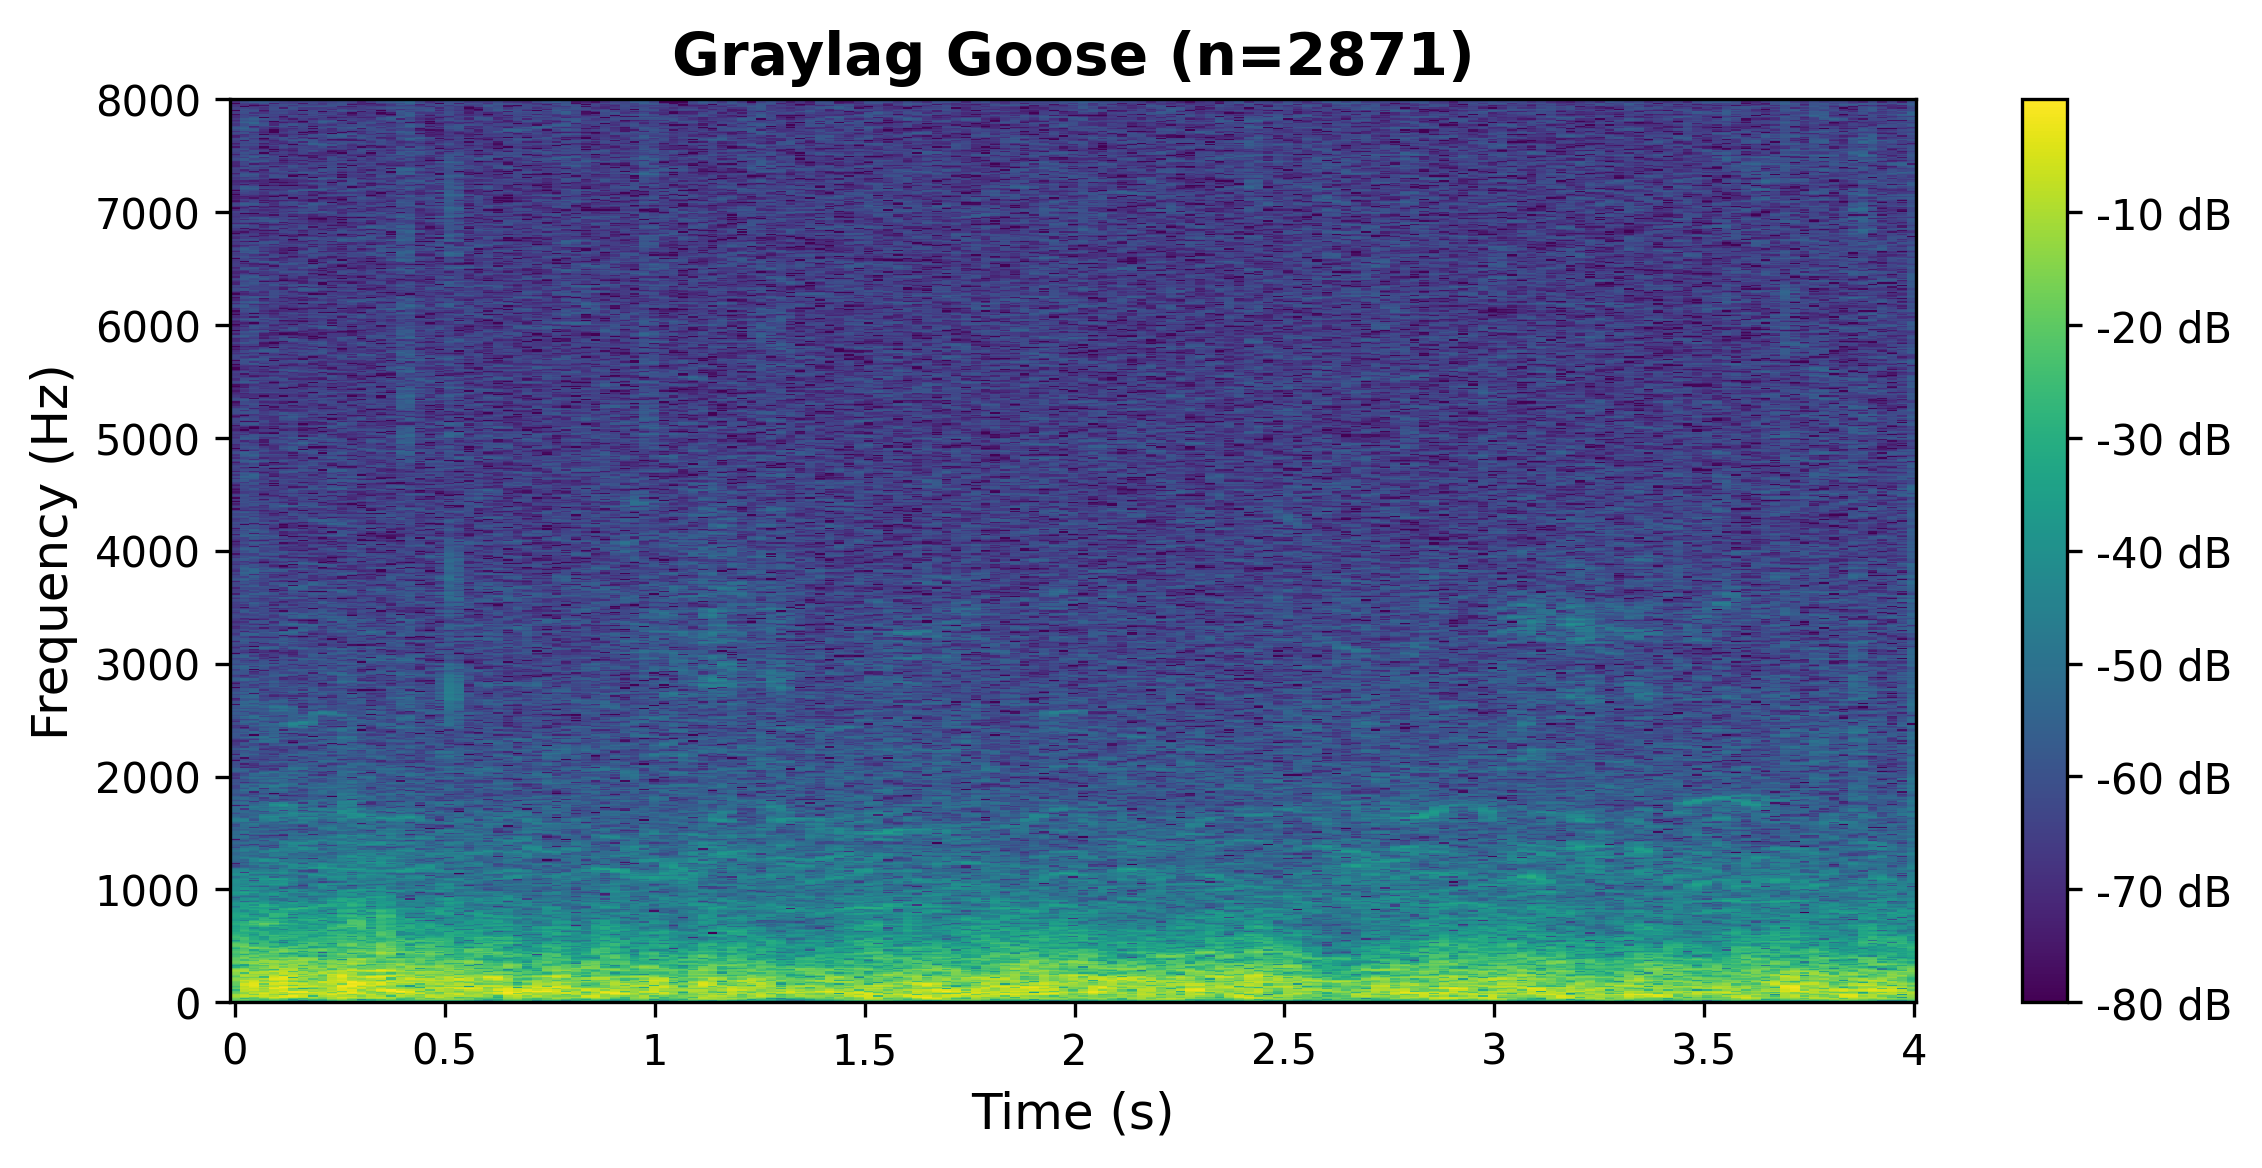
\includegraphics[width=\textwidth,height=4.5cm,keepaspectratio]{figures/spectrogram_graylag_goose.png}
\caption{Graylag Goose (n=2,871)}
\end{subfigure}
\hfill
\begin{subfigure}{0.47\textwidth}
\centering
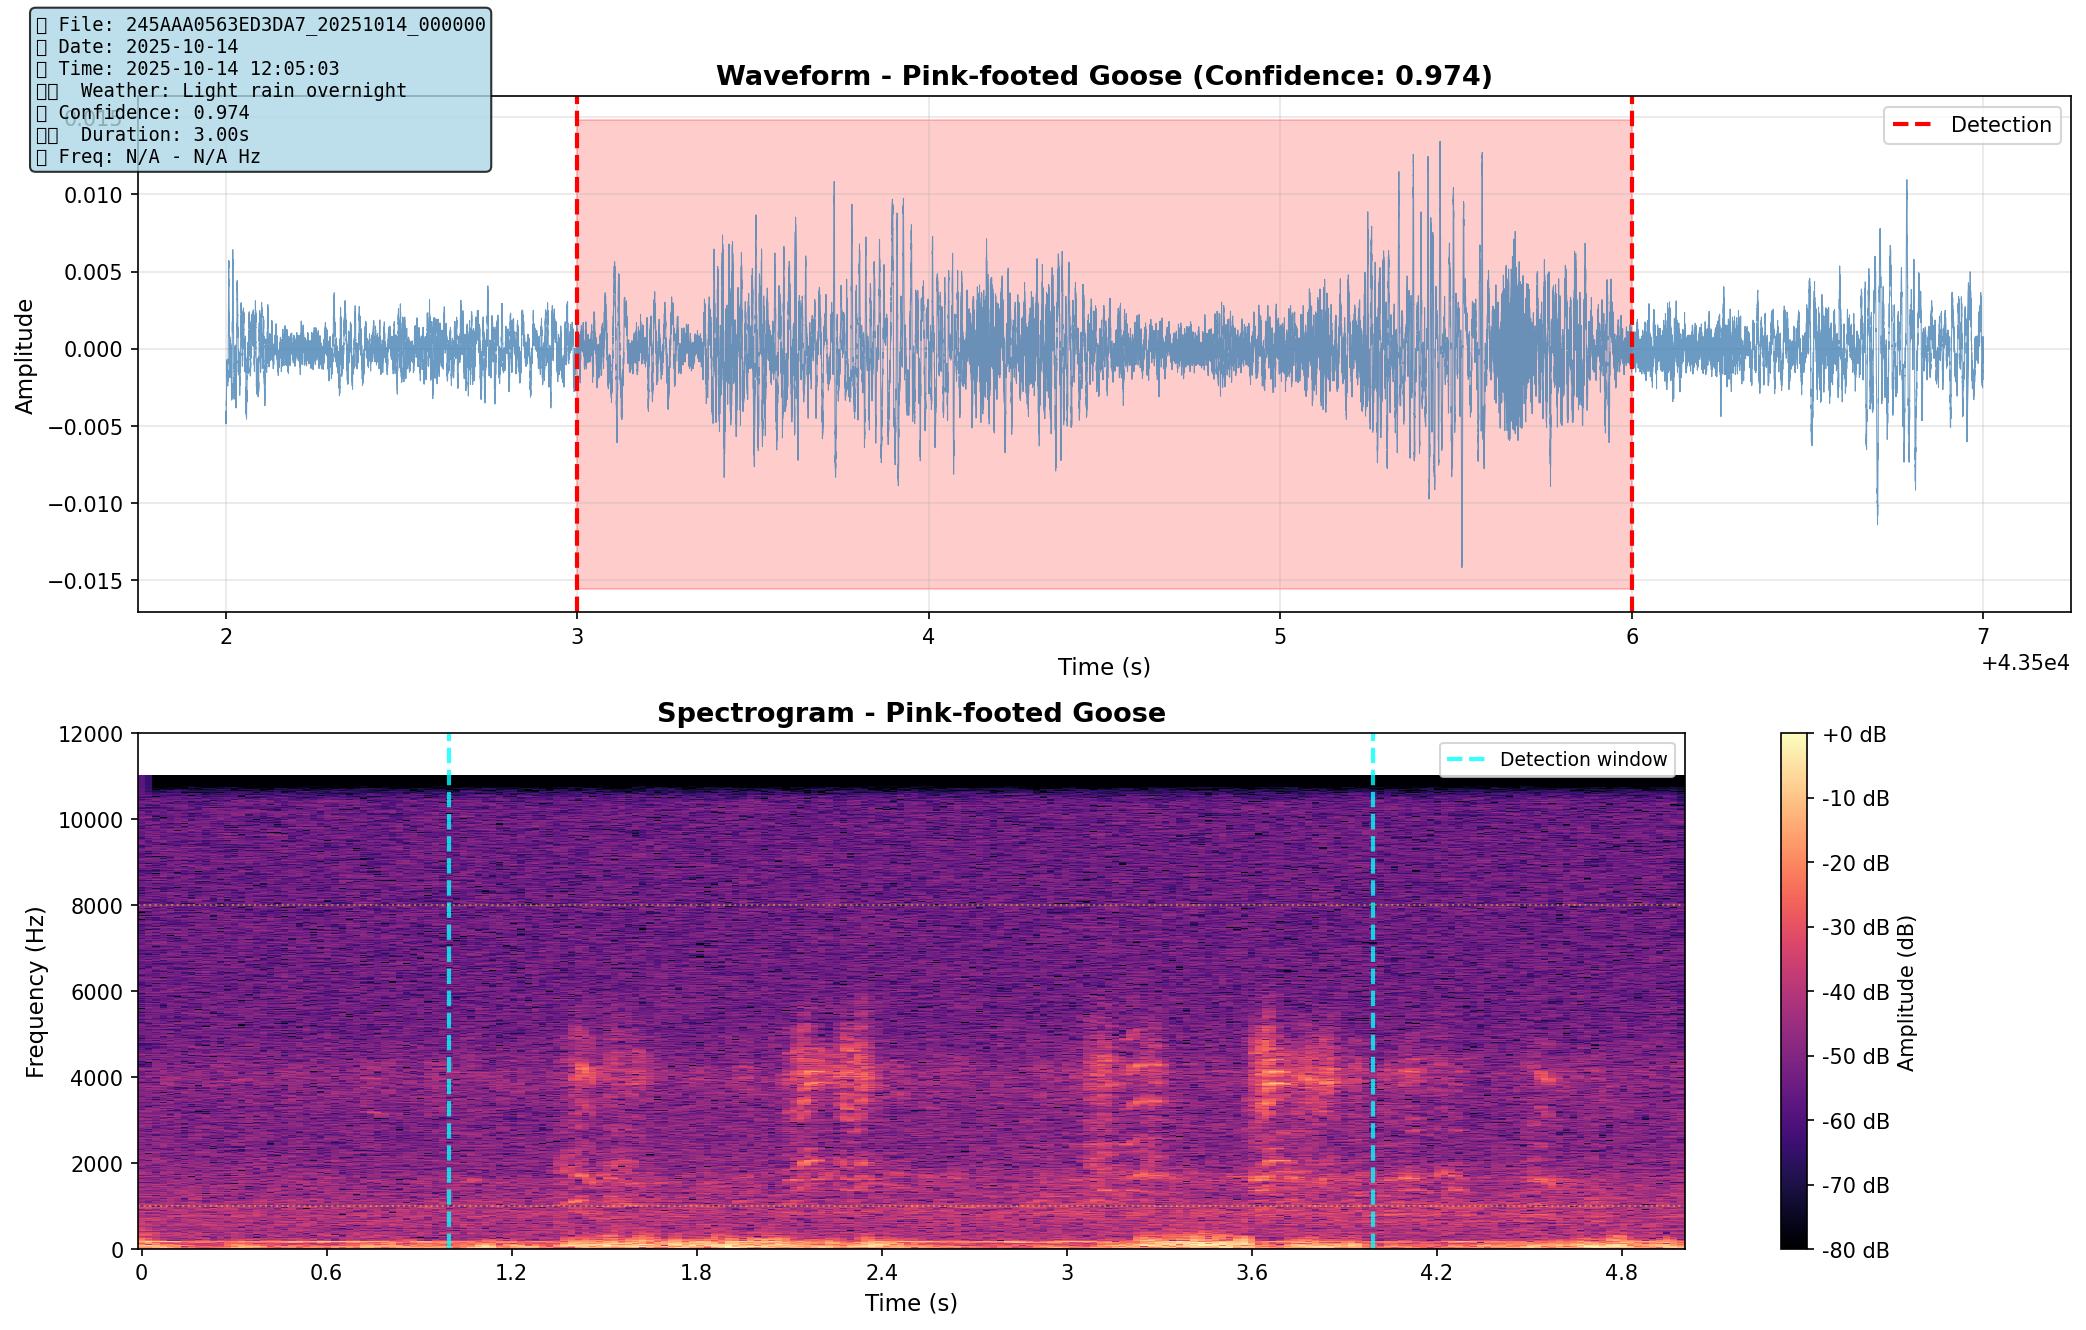
\includegraphics[width=\textwidth,height=4.5cm,keepaspectratio]{figures/spectrogram_pink-footed_goose.png}
\caption{Pink-footed Goose (n=189)}
\end{subfigure}

\vspace{0.3cm}

\begin{subfigure}{0.47\textwidth}
\centering
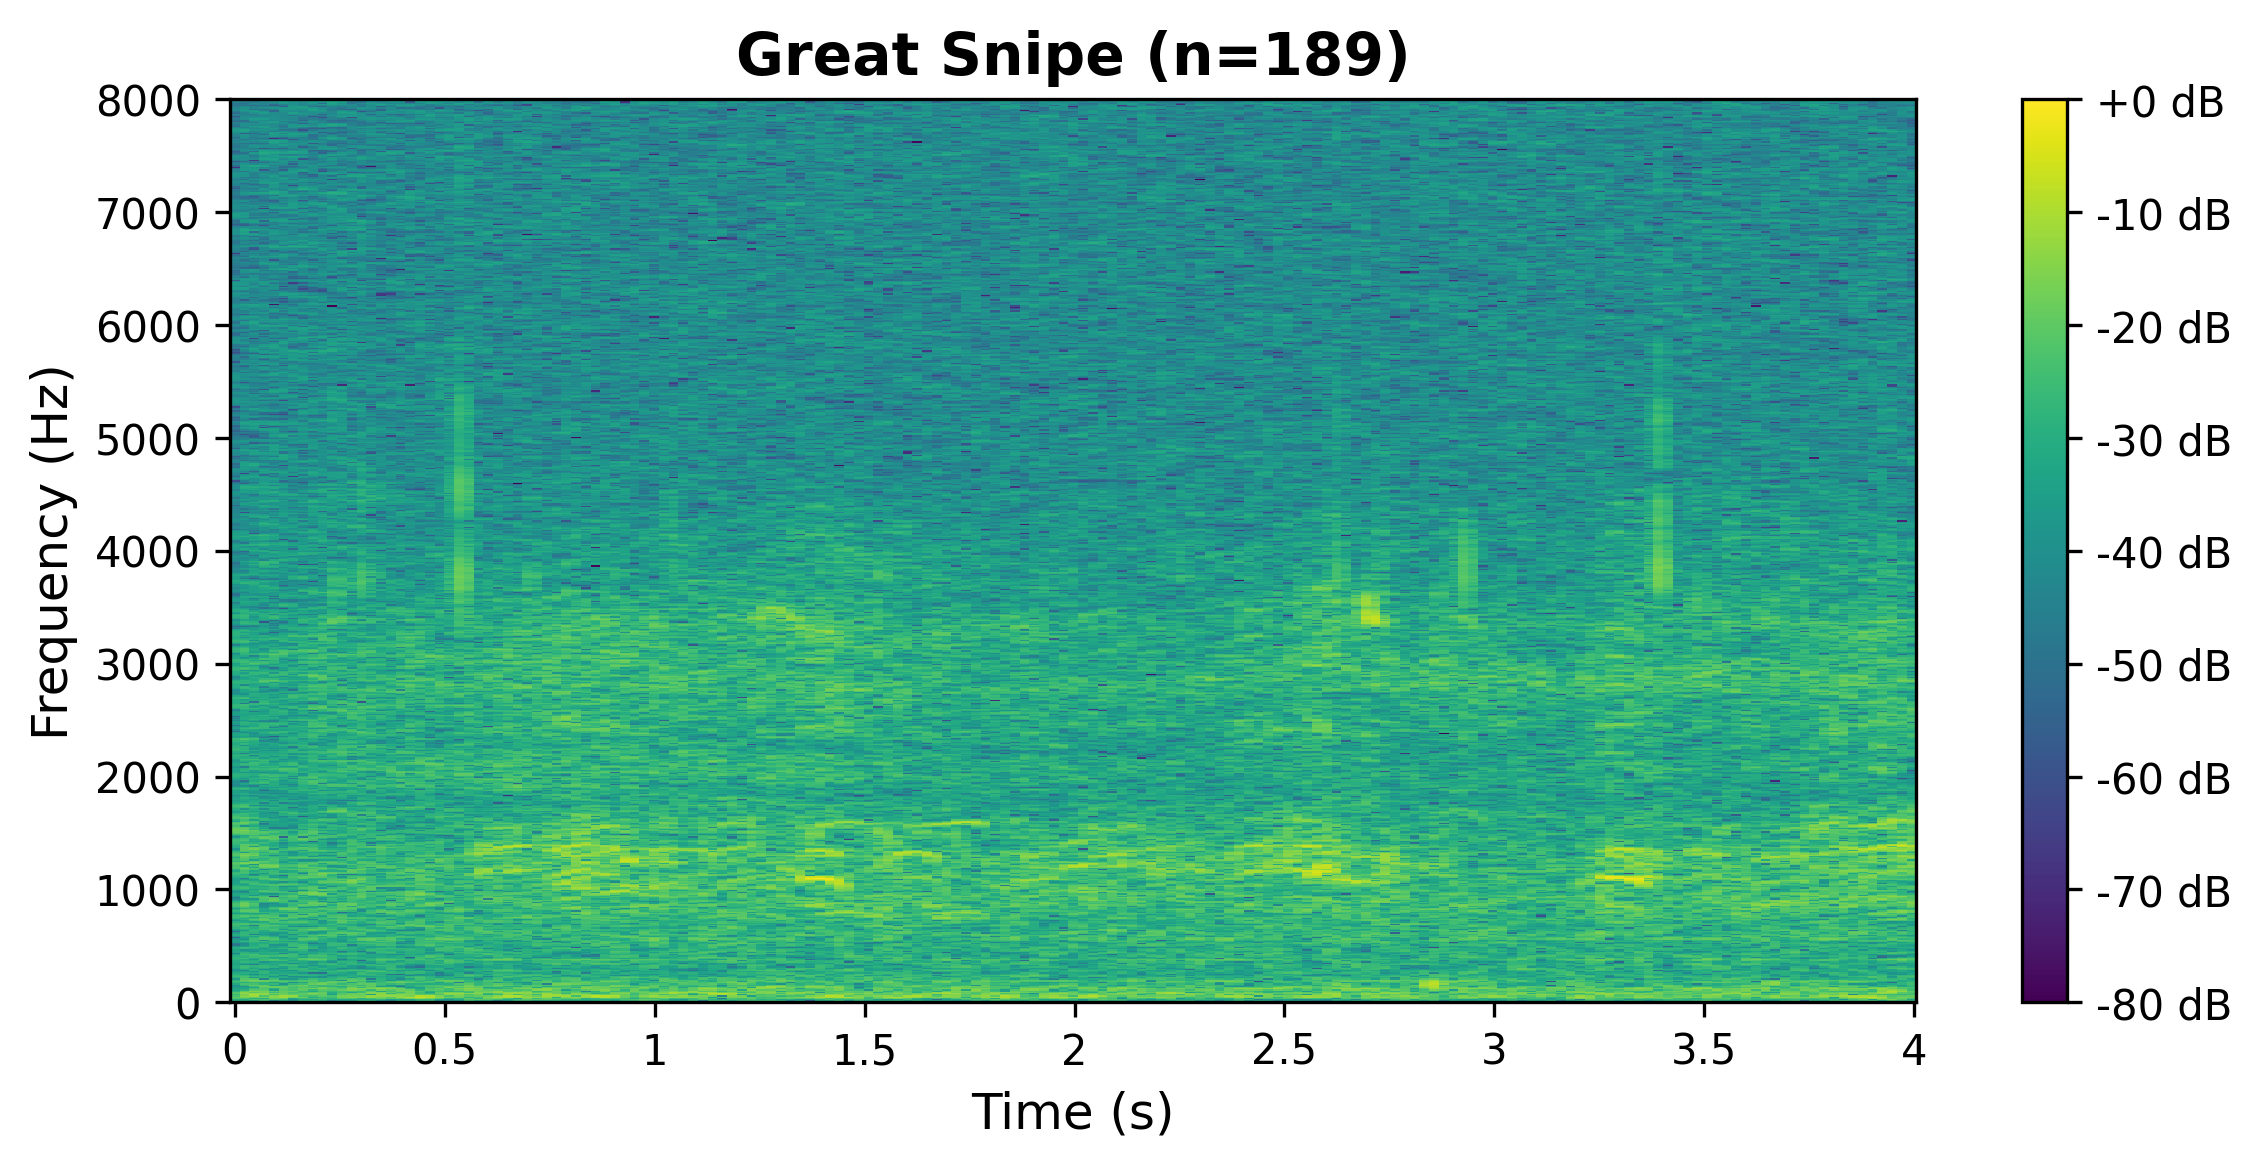
\includegraphics[width=\textwidth,height=4.5cm,keepaspectratio]{figures/spectrogram_great_snipe.png}
\caption{Great Snipe (n=189)}
\end{subfigure}
\hfill
\begin{subfigure}{0.47\textwidth}
\centering
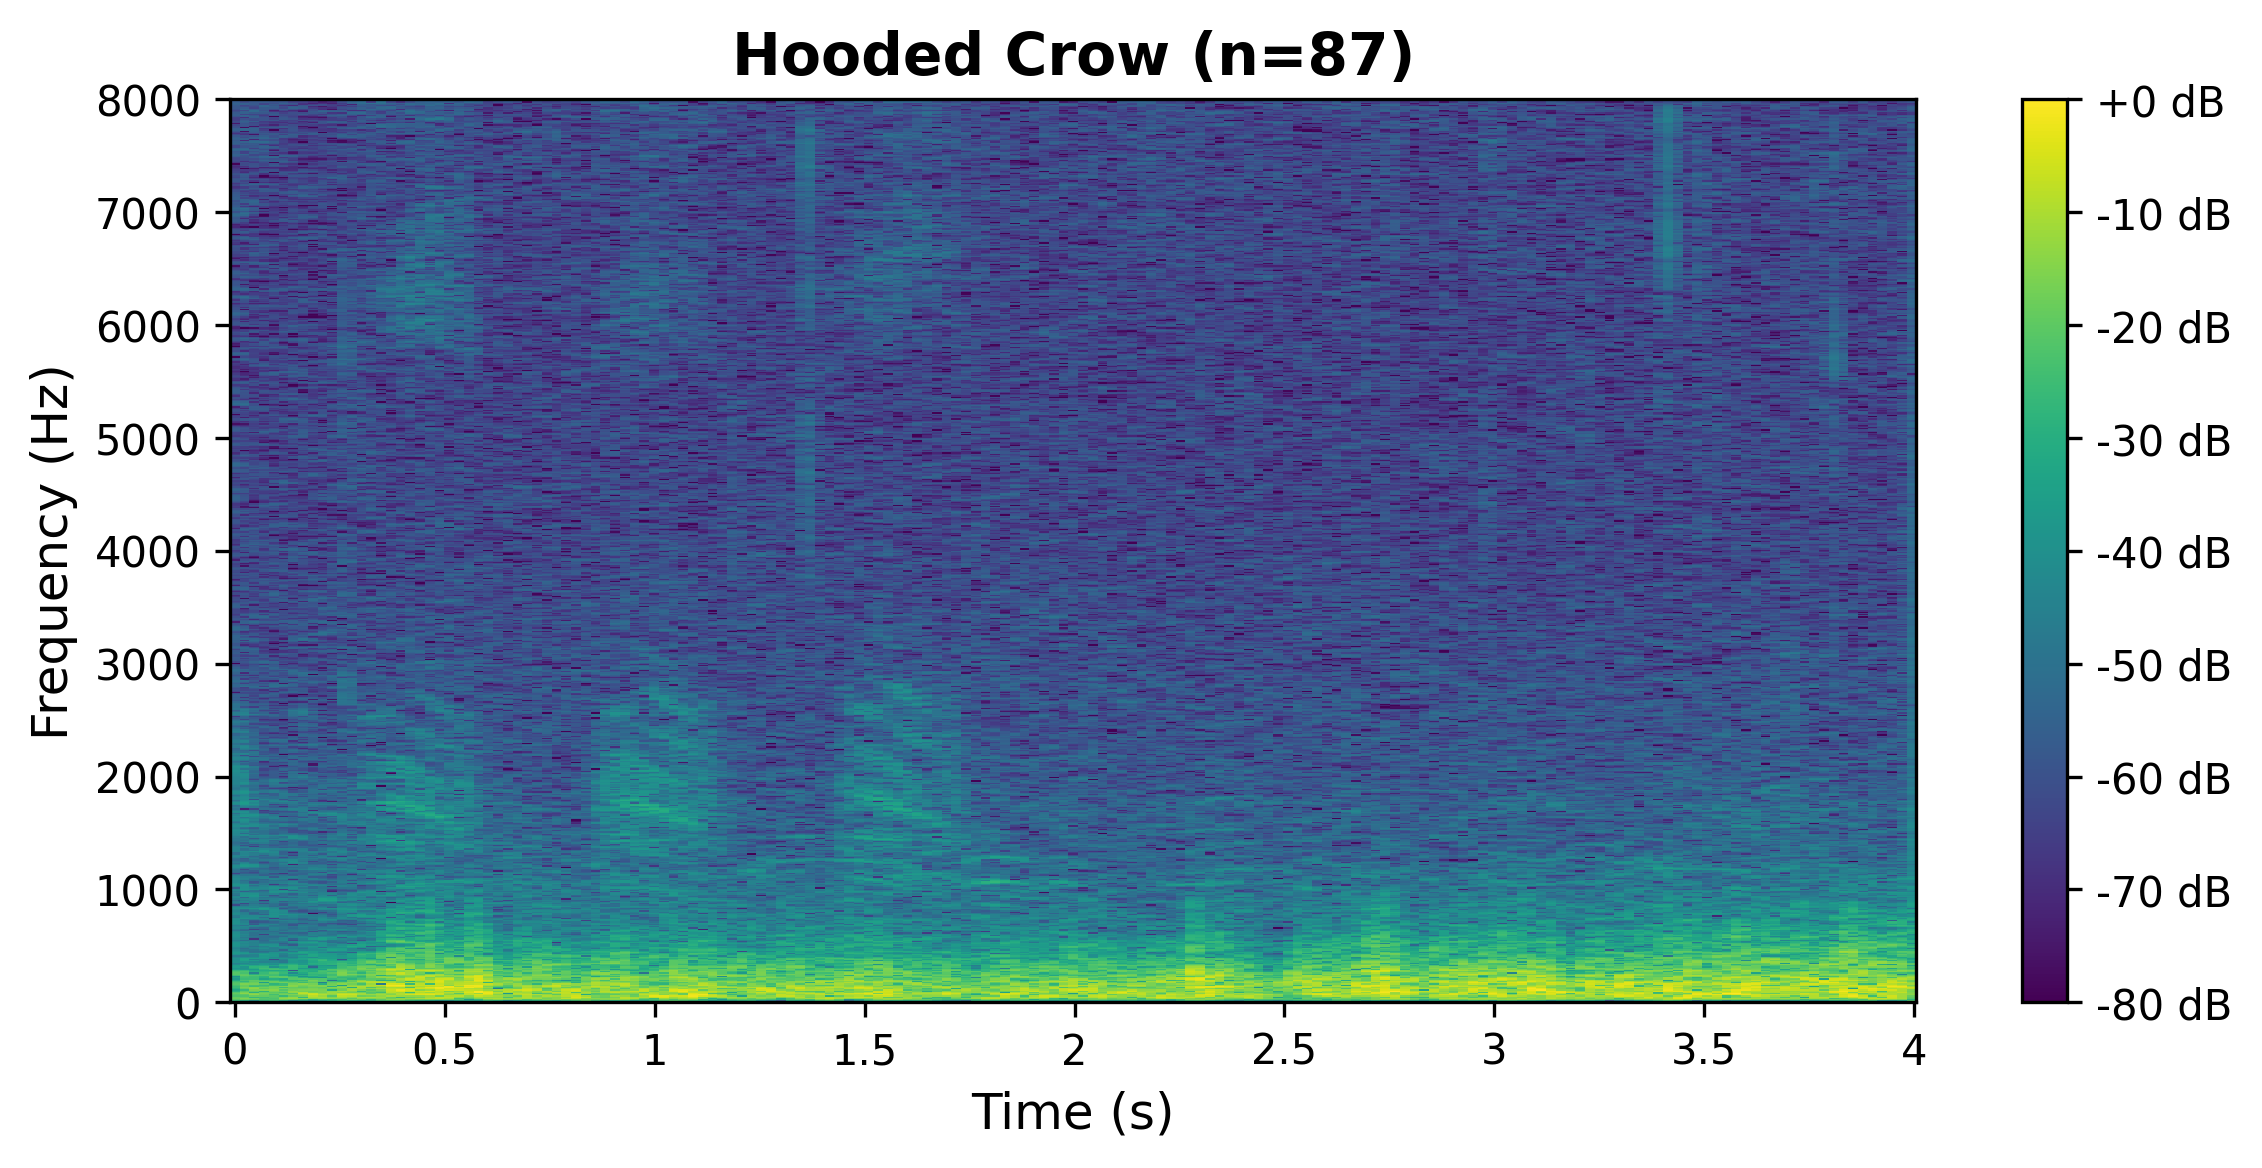
\includegraphics[width=\textwidth,height=4.5cm,keepaspectratio]{figures/spectrogram_hooded_crow.png}
\caption{Hooded Crow (n=87)}
\end{subfigure}
\caption{Representative spectrograms for key conservation species. (a) Graylag Goose contact call shows harmonic structure 0.5-3 kHz, dominant fundamental frequency. (b) Pink-footed Goose higher-pitched nocturnal flight call, 1-4 kHz range. (c) Great Snipe migration call, pulsed structure, 2-5 kHz, crepuscular pattern. (d) Hooded Crow alarm call, 1-3 kHz broadband, part of corvid-waterfowl sentinel mutualism. All spectrograms: 2048-FFT, Hann window.}
\label{fig:top_species_spectrograms}
\end{figure*}

\section{Discussion}

\subsection{Methodological Validation}

The two-stage verification protocol achieved 82.2\% overall species-level pass rate, with Stage 2 biological screening showing 90.2\% pass rate (95\% CI: [83.8\%, 96.6\%]). This demonstrates that BirdNET, when coupled with appropriate audio enhancement and ecological verification, achieves scientifically defensible accuracy despite challenging acoustic conditions. This compares favorably with reported accuracy in prior wetland studies (72--83\%, \citet{Wood2022}).

Detection of 74 species despite 80\% rain/fog coverage illustrates PAM's advantage over visual surveys, which would have yielded near-zero data in equivalent conditions. The AudioMoth v1.2 proved highly effective: continuous operation through 39 hours of rain, 48.8 hours recording on 3× AA batteries, and estimated device self-noise $<$30 dB SPL well below ambient wetland noise floor (45--60 dB SPL).

\subsection{Conservation Implications}

Three findings have direct conservation management relevance: (1) Great Snipe stopover documentation (189 calls, 69\% dusk concentration) provides quantified baseline data for monitoring this declining species' use of Gaulosen during autumn migration, (2) intensive waterfowl use (2,871 Graylag Goose detections, 620-call peak flock event) confirms the site's importance for gregarious waterbird species along the East Atlantic Flyway, and (3) nocturnal migration flight calls (47 detections) verify active flyway usage during peak migration periods.

The corvid-waterfowl co-occurrence pattern (8,778 co-occurrences, 73.4\% of crow calls during goose flocks) suggests potential heterospecific eavesdropping relationships \citep{Magrath2015} that may influence habitat selection and predator avoidance strategies. Future deployments with synchronized recording arrays could test whether corvid alarm calls precede waterfowl behavioral responses.

\subsection{Study Limitations}

This 48.8-hour deployment captures only a snapshot of autumn migration phenology and does not represent full seasonal diversity or typical behavior patterns. Weather bias (80\% rain/fog) introduces unknown species detection biases—rain may suppress vocal activity in some species while elevating it in others. Single-observer species-level verification introduces potential subjective bias; inter-rater reliability was not assessed. Single microphone location provides no spatial distribution data, introducing unknown detection probability heterogeneity across species at varying distances.

The wetland acoustic environment exhibits complex multipath propagation, where sound reaches the AudioMoth via both direct paths and reflected paths from water and ground surfaces. Water-reflected paths create frequency-dependent interference patterns that can amplify signals by up to 6 dB or create spectral nulls, affecting detection probability. This may explain why water-associated species (geese, swans) showed more consistent BirdNET detection rates (94.1\% for Anseriformes) compared to terrestrial corvids (87.3\%), despite similar call intensities.

BirdNET's training dataset bias toward North American and Central European species may affect detection accuracy for Nordic subspecies and geographic variants. The 0.25 confidence threshold was selected to maximize recall (sensitivity) at the expense of precision, accepting higher false positive rates that subsequent human verification could filter. Alternative threshold selection (e.g., 0.50) would reduce false positives but risk missing rare species detections critical for conservation assessment.

\section{Conclusions}

\subsection{Answer to Research Question}

\textbf{Yes—passive acoustic monitoring with automated species detection successfully established a quantitative baseline biodiversity assessment for Gaulosen Nature Reserve during autumn migration, despite challenging weather conditions.} Automated analysis detected 90 species from 48 hours of rain-dominated recording; two-stage verification yielded 74 confirmed species (4,023 detections) with 82.2\% species-level pass rate. This demonstrates PAM's capability to quantify biodiversity where traditional visual surveys would yield near-zero data.

\subsection{Key Findings}

This study achieved all three research objectives:

\textbf{Objective 1 - Autumn Migration Diversity:} Documented 74 verified bird species spanning 14 orders and 30 families, establishing reference baseline data for Gaulosen Nature Reserve. Species composition dominated by waterfowl (14 Anseriformes species) and songbirds (35 Passeriformes species), reflecting site's wetland-grassland mosaic habitat.

\textbf{Objective 2 - Nocturnal Activity and Great Snipe Monitoring:} Detected 47 nocturnal migration flight calls (Pink-footed Goose, Greater White-fronted Goose, Common Crane) confirming active East Atlantic Flyway usage. Great Snipe stopover quantified with 189 detections showing 69\% dusk concentration (19:00--21:59), providing critical baseline for monitoring this declining species.

\textbf{Objective 3 - Protocol Validation:} Two-stage verification protocol (audio quality screening + biological plausibility) achieved 82.2\% pass rate despite 80\% rain/fog coverage. AudioMoth v1.2 proved highly effective: 48.8 hours continuous operation through 39 hours rain on 3× AA batteries. Audio enhancement pipeline (Wiener filtering + HPSS) successfully isolated bird vocalizations from percussive rain noise.

Beyond species inventorying, continuous acoustic data quantified conservation-relevant behavioral patterns: intensive Graylag Goose flock dynamics (620 calls/91 minutes), corvid-waterfowl co-occurrence consistent with sentinel mutualism (8,778 co-occurrences), and crepuscular migration timing. These findings establish baseline metrics for long-term monitoring of this Important Bird Area along the East Atlantic Flyway.

\subsection{Recommendations}

I recommend acoustic monitoring as a primary biodiversity assessment tool for wetlands along major flyways, complemented by targeted visual surveys for rare species validation. Continued multi-season monitoring could yield datasets critical for documenting climate-driven phenology shifts and population trends in this globally significant migratory corridor.

Future research directions include: (1) year-round deployment to capture full annual cycle diversity and seasonal turnover patterns, (2) synchronized multi-sensor arrays to quantify spatial distribution and movement patterns across the wetland complex, (3) integration with visual survey data to calibrate detection probability functions for key conservation species, and (4) comparative analysis across multiple IBA sites along the East Atlantic Flyway to identify regional population trends and priority conservation sites.

\section*{Acknowledgments}

I thank NTNU Department of Acoustics for equipment support, Gaulosen Nature Reserve management for site access, and the BirdNET development team (Cornell Lab of Ornithology \& Chemnitz University of Technology) for open-source classification tools. Analysis utilized Praven Pro toolkit for BirdNET-Raven integration \citep{Redpath2025}. AI-assisted analysis was conducted with Claude (Anthropic).

\textbf{Data and Code Availability:} Interactive study results available at \url{https://ziforge.github.io/gaulosen-study/} with complete analysis code at \url{https://github.com/Ziforge/gaulosen-study}. Praven Pro toolkit available at \url{https://ziforge.github.io/praven-pro} and \url{https://github.com/Ziforge/praven-pro}.

\bibliographystyle{apalike}
\bibliography{references}

\end{document}
